%%%%%%%%%%%%%%%%%%%%%%%%%%%%%%%%%%%%%%%%% 
%               Template                %
%          kindly provided by           %
%             Daniel Regado             %                 
%%%%%%%%%%%%%%%%%%%%%%%%%%%%%%%%%%%%%%%%% 

\documentclass[12pt, a4paper]{report} % Page and font size
\setlength{\parindent}{0.5cm}

% Packages
\usepackage[margin=1in]{geometry}
\usepackage{graphicx}
\usepackage{fontspec}
\usepackage{multirow}
\usepackage{afterpage}
\usepackage{layout}
\usepackage{xcolor}
\usepackage{color}
\usepackage{caption}
\usepackage{fix-cm}
\usepackage{float}
\usepackage{makecell}
\usepackage{tabularx}
\usepackage{titlesec}
\usepackage{pdfpages}
\usepackage{longtable}
\usepackage[english]{babel}
\usepackage{setspace}
\usepackage[square, numbers]{natbib}
\bibliographystyle{abbrvnat}
\usepackage{hyperref}
\usepackage{bookmark}
\usepackage[acronym, shortcuts, style=index]{glossaries}

\makeglossaries
\usepackage{subcaption}
\usepackage[title]{appendix}
% \usepackage{multico}

\usepackage{beton}
\usepackage{amsmath}
\usepackage{amsthm}
\usepackage{amssymb}
% \usepackage{algorithm}
% \usepackage{algpseudocode}
\usepackage{fancyhdr}
\usepackage{comment}
\usepackage{cleveref}

% \usepackage{minted}
\usepackage[inline]{enumitem}
\usepackage[normalem]{ulem}
\usepackage{soul}

\usepackage{listings}

\usepackage{ebproof}
\usepackage{tikz-cd}

\newcommand{\LamM}{\pmb{\lambda m}}
\newcommand{\LamVM}{\pmb{\vec \lambda m}}

\newcommand{\Lam}{\pmb{\lambda}}
\newcommand{\LamV}{\pmb{\vec \lambda}}


% Definitions, Lemmas and Theorems
\newtheorem{theorem}{Theorem}
\crefname{theorem}{Theorem}{Theorems}
\newtheorem{lemma}{Lemma}
\crefname{lemma}{Lemma}{Lemmas}
\newtheorem{claim}{Claim}
\crefname{claim}{Claim}{Claims}

\newtheorem{definition}{Definition}
\crefname{definition}{Definition}{Definitions}

\newtheorem{corollary}{Corollary}

\newtheorem*{notation}{Notation}
\newtheorem*{remark}{Remark}
\crefname{remark}{Remark}{Remarks}
\newtheorem*{convention}{Convention}

% Global counters (don't reset on chapter)
\counterwithout{figure}{chapter}
\counterwithout{table}{chapter}
\counterwithout{equation}{chapter}

% Colors
\definecolor{darkBlue}{cmyk}{1.0, 1.0, 0.0, 0.1}
\definecolor{darkGreen}{cmyk}{1.0, 0.0, 1.0, 0.4}
\definecolor{navyBlue}{cmyk}{1.0, 1.0, 0.0, 0.1}

\hypersetup{
  bookmarksnumbered=true,
  plainpages=false,
  pdffitwindow=true,
  pdfauthor={Daniel Regado},
  pdfcreator={Daniel Regado},
  pdfproducer={Daniel Regado},
  colorlinks=true,
  linkcolor=darkBlue,
  citecolor=darkGreen,
  filecolor=magenta,
  urlcolor=navyBlue
}

% UMinho formatting
\onehalfspacing % 1.5 spacing
\geometry{ % Page borders
  a4paper,
  right=25mm,
  rmargin=0mm,
  outer=25mm,
  left=0mm,
  lmargin=0mm,
  inner=25mm,
  top=0mm,
  tmargin=25mm,
  bottom=0mm,
  bmargin=25mm
}
\setmainfont[Ligatures=TeX, AutoFakeSlant=0.20, BoldFont=NewsGotTBold.ttf]{NewsGotT.ttf} % NewsGotT font

% Titles formatting
\titleformat{\chapter}[display]{\normalfont\bfseries\color{darkgray}}{\chaptertitlename\ \thechapter}{0pt}{\Large}
\titleformat*{\section}{\color{darkgray}\Large\bfseries}
\titleformat*{\subsection}{\color{darkgray}\Large\bfseries\color{darkgray}}
\titleformat*{\subsubsection}{\color{darkgray}\Large\bfseries}
\setcounter{secnumdepth}{3}
\renewcommand{\thesubsubsection}{\alph{subsubsection})}
\titlespacing{\chapter}{0pt}{-40pt}{20pt}

% Settings for headers and footers
\pagestyle{fancy}
\fancyhf{}
\fancyfoot[C]{\thepage}
\setlength{\headheight}{15pt}
\renewcommand{\headrulewidth}{0.0pt}

% Header for Abstract and Resumo
\fancypagestyle{title_on_header}{
  \fancyhead[C]{\textit{Your Title Goes Here}}
  \fancyfoot[C]{\thepage}
}

% lstlisting coq style (inspired from a file of Assia Mahboubi)
\newcommand{\lst}{\lstinline}
\lstdefinelanguage{Coq}%
  {morekeywords={Variable,Inductive,CoInductive,Fixpoint,CoFixpoint,%
      Definition,Lemma,Theorem,Axiom,Local,Save,Grammar,Syntax,intro,%
      trivial,Qed,intros,Symmetry,Simpl,Rewrite,apply,elim,assumption,%
      left,Cut,Case,auto,unfold,exact,right,Hypothesis,Pattern,destruct,%
      constructor,Defined,Fix,Record,Proof,induction,Hints,exists,let,in,%
      Parameter,split,Red,reflexivity,transitivity,if,then,else,Opaque,%
      Transparent,inversion,Absurd,Generalize,Mutual,Cases,of,end,Analyze,%
      AutoRewrite,Functional,Scheme,params,Refine,using,discriminate,Try,%
      Require,Load,Import,Scope,Set,Open,Section,End,match,with,Ltac,%
      Instance,%
      bind,as,%
      % , exists, forall
	},%
   sensitive, %
   morecomment=[n]{(*}{*)},%
   morestring=[d]",%
   literate={=>}{{$\Rightarrow$}}1 {>->}{{$\rightarrowtail$}}2{->}{{$\rightarrow$}}1
   {\/\\}{{$\wedge$}}1
   {|-}{{$\vdash$}}1
   {\\\/}{{$\vee$}}1
   {~}{{$\sim$}}1
   {exists}{{$\exists\!\!$}}1
   {forall}{{$\forall\!\!$}}1
   {beta1}{{$\beta_1$}}1
   {beta2}{{$\beta_2$}}1
   {sigma}{{$\sigma$}}1
   {theta}{{$\theta$}}1
   {tau}{{$\tau$}}1
   {rho}{{$\rho$}}1
   {xi}{{$\xi$}}1
   {exi}{exi}3 % insufficient patch to print reflexivity correctly
   {zeta}{{$\zeta$}}1
   {Gamma}{{$\Gamma$}}1
   {Delta}{{$\Delta$}}1
   {\\rhd}{{$\rhd$}}1
   %{>>}{\scomp}1
   %{<>}{{$\neq$}}1 indeed... no.
  }[keywords,comments,strings]%

\lstset{
   basicstyle=\ttfamily,
   keywordstyle=\bfseries\color{blue}
  }
\lstset{language=Coq}
\lstset{columns=fullflexible, keepspaces}

% *******************************************************************

\begin{document}
\newacronym{um}{UM}{University of Minho} % Import acronyms

% Title and Cover Page
% The files need to be changed and exported from Adobe Illustrator
% Adobe Illustrator files are in front/cover/illustrator
\begin{titlepage}
  % 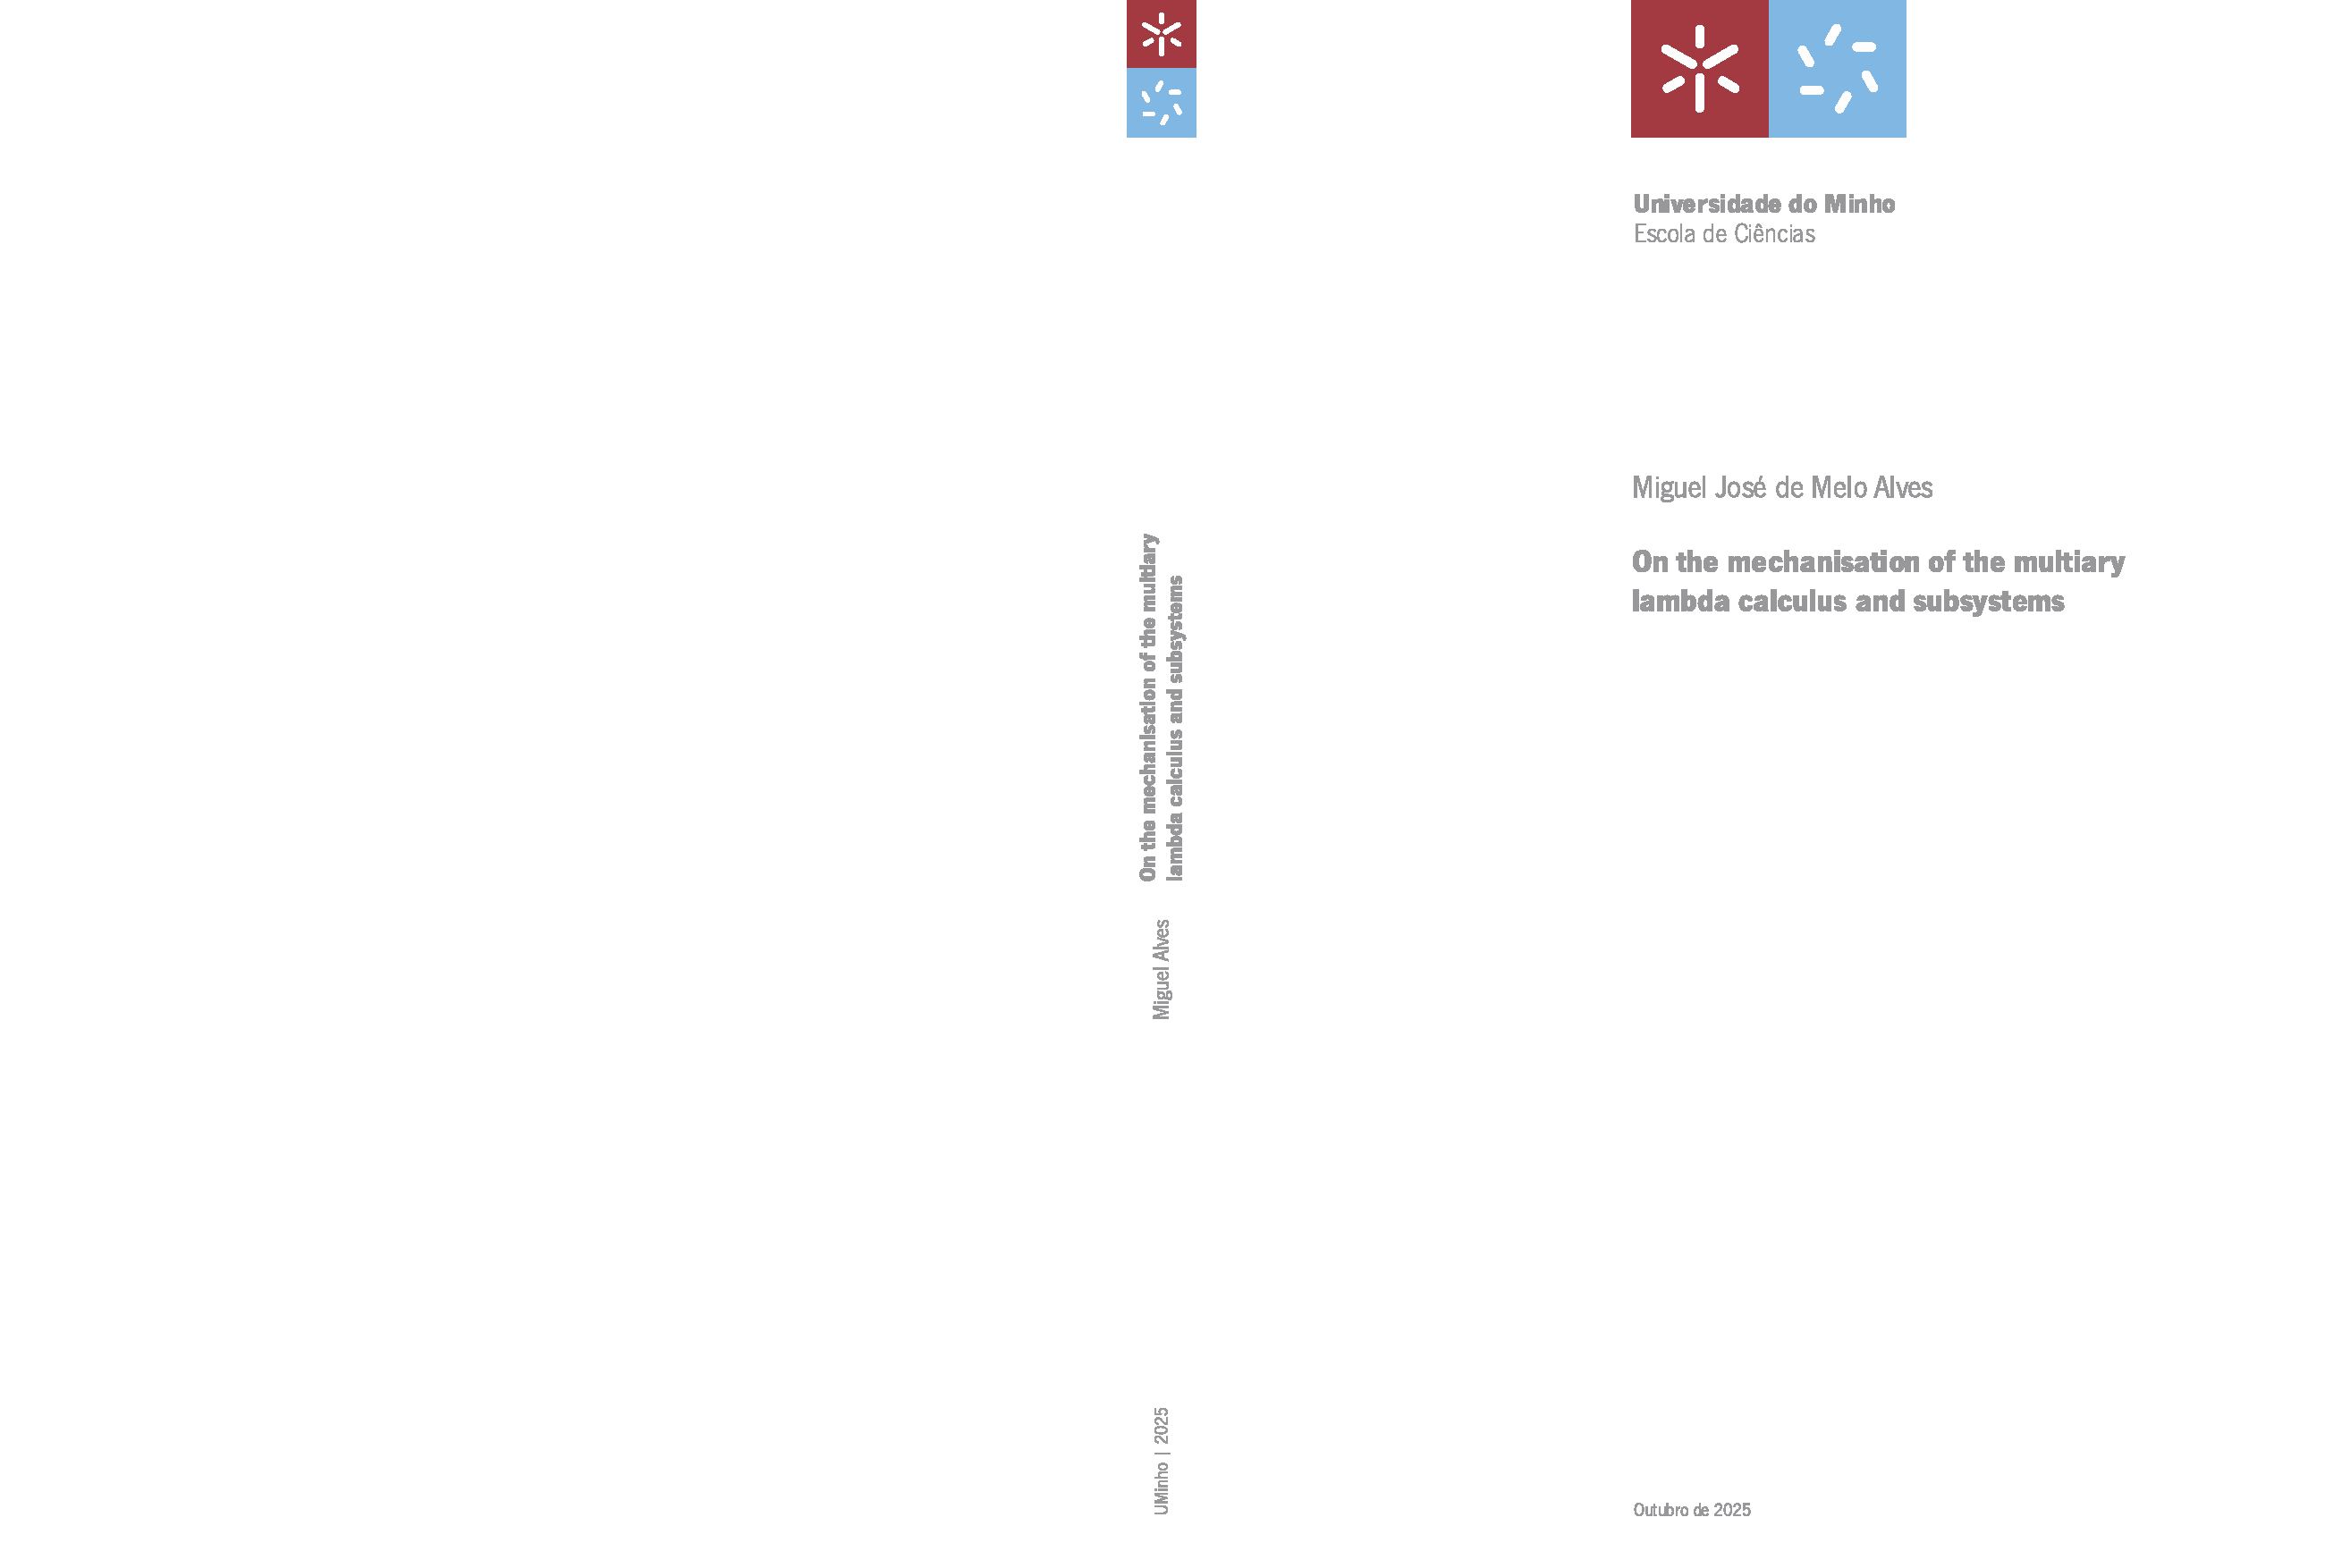
\includepdf[pages={1,2}, fitpaper]{front/cover/title.pdf}
  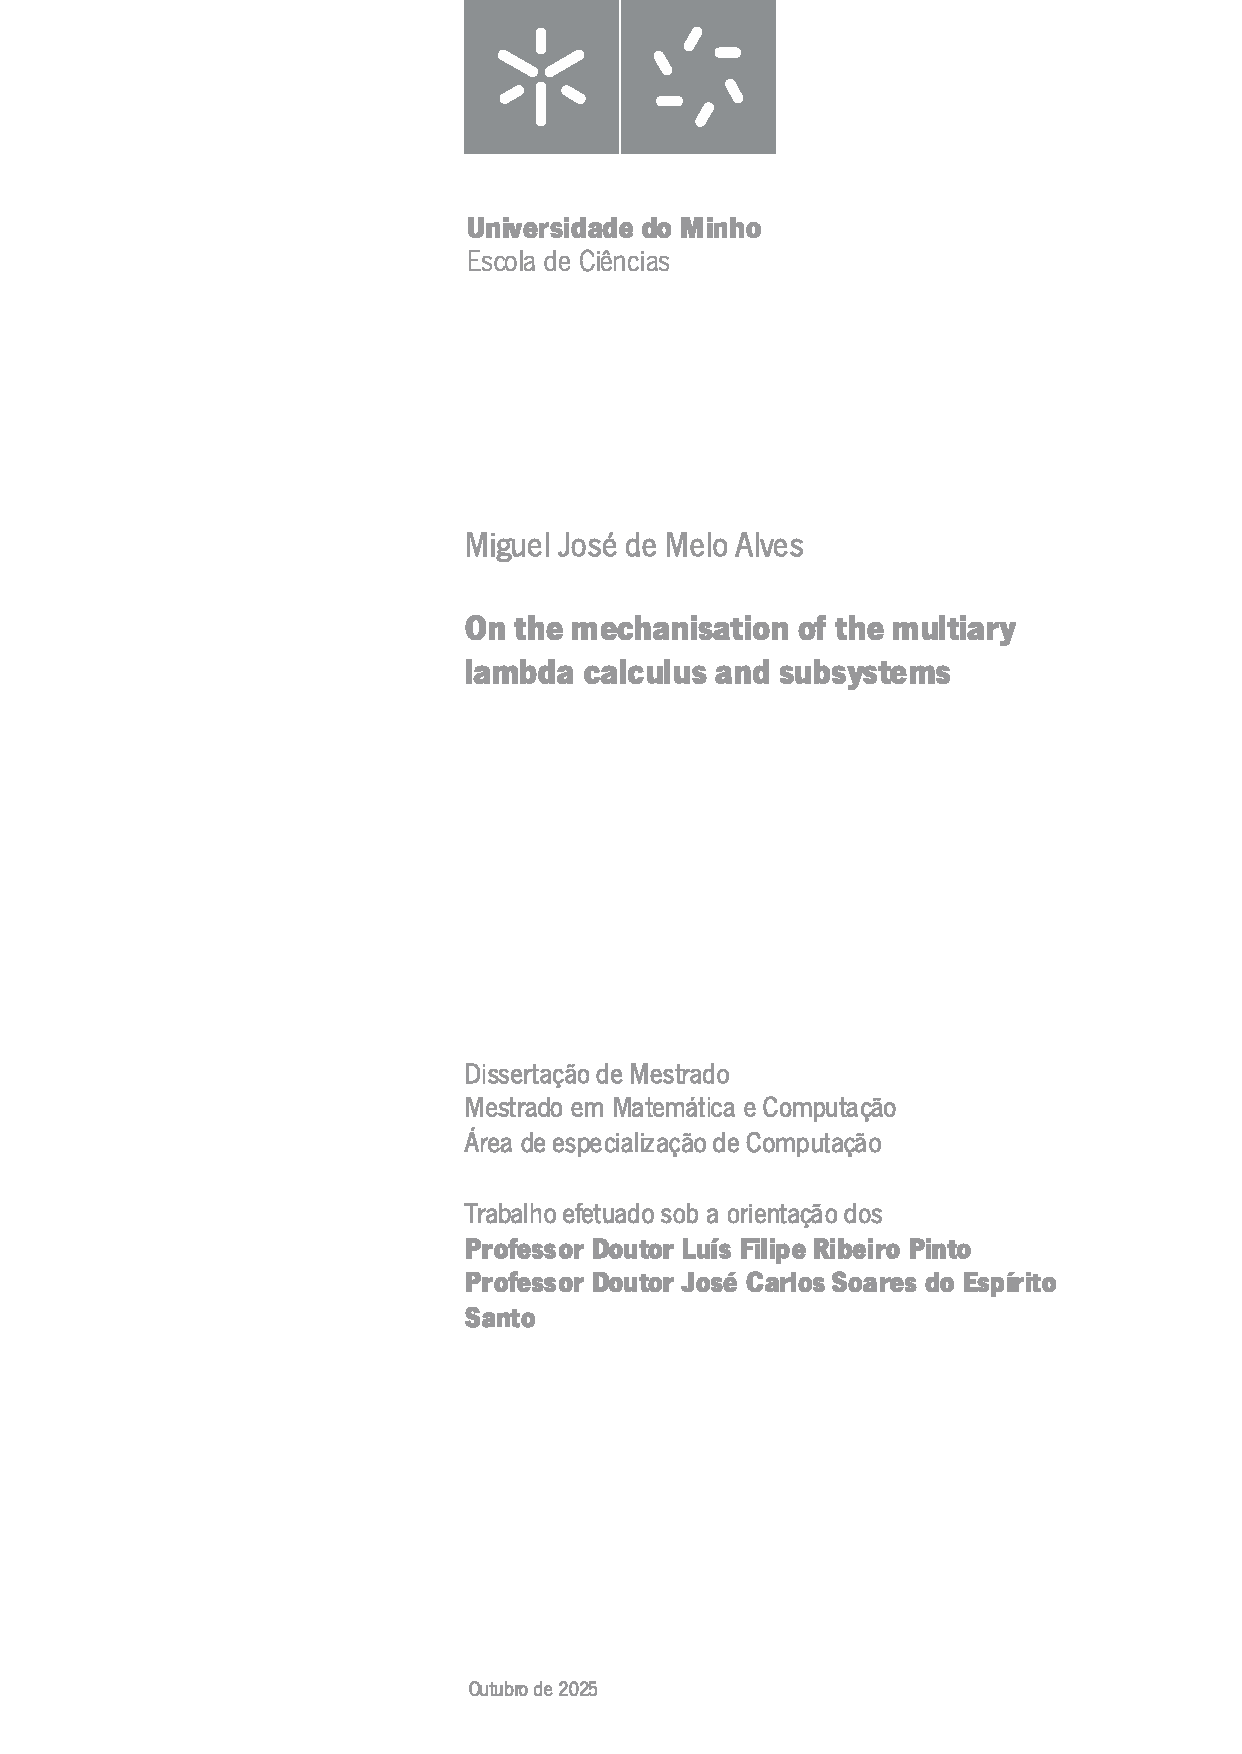
\includepdf{front/cover/cover.pdf}
\end{titlepage}

% Front matter
\pagenumbering{roman}
\setcounter{page}{2} % Cover page is the first page, but not numbered
% \include{front/copyright}\clearpage
% \chapter*{Acknowledgments}

I feel blessed to write this, as I contemplate so many people that I have to thank, as I see so many people that I love and love me back.

First and foremost, I must thank my family for allowing me to pursue what I love and for unconditionally supporting my passions.

Second, I want to deeply thank my girlfriend Inês for being my companion throughout this year of confusion, tiredness and grumpiness.
I still owe you a complete explanation of what $\Lam$-calculus is.

Third, I want to thank all my friends...should I name them?
To Nando, Marco and David, as you are a second kind of girlfriend to me.
To Gaspar, Rodrigo and Kiko, as you have known me for a long time and part of who I am today is because of you.
To Pepa, as you may not understand how much of a help you were to me throughout this year.
To Gui, Zé, Bruno, Sofia, Manada, Gonçalo, Jason, Jonny and to every algebra class that made us closer.
To Faustino, Ricardo, Guilherme and Filipa, for making me feel more at home in Braga.
To my long time friends, Couves e Beterrabas, for being with me in such an important and playful time in my life.
To my CVX group, VitaminaC, for walking with me.
To CREU, Missão País, Fonte da Prata and to every friend that I have made in those special places - a piece of my heart lies with each of you.

Fourth and last, I want to thank everyone who I feel had a part in my logical education, from Rola and Rita to professor Filipe and professora Alice Viveiros.
And, of course, to my kind supervisors.
Thank you, Professor Luís, for your patience and for your focused, optimistic and close help throughout this joyful process.
Thank you, Professor José Carlos, for your enthusiasm and for every exciting conversation we have shared.

To everyone that casually asked what I was studying in my dissertation and kept their attention at my explanation - because attention without distraction is a prayer - I thank you.

%%% Local Variables:
%%% mode: LaTeX
%%% TeX-master: "../dissertation"
%%% End:
\clearpage
% \chapter*{Statement of Integrity}
\noindent I hereby declare having conducted this academic work with integrity. I confirm that I have not used plagiarism or any form of undue use of information or falsification of results along the process leading to its elaboration.

\noindent I further declare that I have fully acknowledged the Code of Ethical Conduct of the University of Minho.\clearpage
% \chapter*{Resumo}
\thispagestyle{title_on_header}
Abstract em português.

\paragraph{Palavras-chave} 3 a 5 palavras-chave, ordenadas alfabeticamente e separadas por vírgulas\clearpage
% \chapter*{Abstract}
\thispagestyle{title_on_header}

This dissertation details the mechanisation within the \textit{Rocq Prover} of a multiary $\Lam$-calculus (system $\LamM$) and associated metatheory.
We are motivated by the necessity for computer verification of metatheoretical proofs - which are often lengthy and prone to human error in manual treatments - and by the interest to extend the Curry-Howard isomorphism to calculi whose typing rules are inspired by the sequent calculus.
Our development uses a de~Bruijn representation to mechanise terms and uses the \textit{Autosubst} library to define the desired capture-avoiding substitution operations.
The formalised system $\LamM$ includes its reduction rules, typing system and core theorems like subject reduction.
A major contribution was the study of its canonical subsystem, an isomorphism of this subsystem with the simply typed $\Lam$-calculus and a conservativeness result.
Interestingly, by formalising the isomorphism with the $\Lam$-calculus, we were able to derive the confluence for $\LamM$.
This work presents a novel mechanisation of this metatheory and describes the rigorous methodology implemented.

\paragraph{Keywords} $\lambda$-calculus, sequent calculus, proof assistants

%%% Local Variables:
%%% mode: LaTeX
%%% TeX-master: "../dissertation"
%%% End:
\clearpage
% \thispagestyle{plain}
\vspace*{\fill}
\begin{flushright}
\textit{"We adore chaos because we love to produce order."}

\paragraph{}
M. C. Escher
\vspace*{\fill}
\end{flushright}\clearpage
\setcounter{tocdepth}{1} % Only go down to section level on ToC
\tableofcontents\fancyhead[R]{\textit{Contents}}
% \listoffigures\fancyhead[R]{\textit{List of Figures}}
% \listoftables\fancyhead[R]{\textit{List of Tables}}
% \printglossaries\fancyhead[R]{\textit{Acronyms}}

% Header with section number and name
\fancyhead[R]{\rightmark}
\renewcommand{\sectionmark}[1]{\markright{\thesection\ \textit{#1}}}

% Thesis content
\pagenumbering{arabic} % Reset page counter
\chapter{Introduction}
\label{c:intro}


\section{Motivation}
\label{s:motivation}
There is no motivation, yet we need to write one.


\section{Objectives}
\label{s:objectives}
Formalise results about $\lambda$-calculus variants in \textit{Coq}.


\section{Document Structure}
\label{s:doc_structure}
List your chapters here, with a very brief description of each one.

% Include your chapters here
\chapter{Background}
\label{c:background}

% In this chapter, we intend to take the example of formalising some theory about the $\Lam$-calculus as a motivation to display some core aspects involved in the more elaborate formalisations ahead.

The following chapter introduces essential background to aid the reading of this dissertation.
% It will take the scheme used in the subsequent chapters:
% a first part of theoretical presentation and a second part of mechanisation.
First, we introduce the well-known simply typed $\Lam$-calculus.
Then, we delve into the theory on mechanisation of meta-theory, specifically in the context of our work.
These concepts are introduced and motivated by the task of formalising the $\Lam$-calculus system introduced.

\section{Simply typed $\Lam$-calculus}

For the untyped lambda calculus descriptions we refer to \cite{Barendregt1987}.
For what types and the simply typed lambda calculus is about we refer to \cite{Barendregt2013} and \cite{Hindley1997}.

\subsection{Syntax}

\begin{definition}[$\Lam$-terms]
  The $\Lam$-terms are defined by the following grammar:
  \[ M, N \ ::= \ x \ | \ (\lambda x . M) \ | \ (M N) \]
  where $x$ denotes any variable, typically in the range of $x, y, z$.
\end{definition}

\begin{notation}
  We shall assume the usual notation conventions on $\Lam$-terms:

  \begin{enumerate}
  \item Outermost parenthesis are omitted.
  \item Multiple abstractions can be abreviated as $\lambda x y z . M$ instead of  $\lambda x . (\lambda y . (\lambda z . M))$.
  \item Multiple applications can be abreviated as $M N_1 N_2$ instead of $(M N_1) N_2$.
  \end{enumerate}
\end{notation}

\begin{definition}[Free variables]
  For every $\Lam$-term $M$, we recursively define the set of free variables in $M$, $FV(M)$, as follows:  
  \begin{align*}
    & FV( x ) = \{ x \}, \\
    & FV( \lambda x . M ) = FV(M) - \{ x \}, \\
    & FV( M N ) = FV(M) \cup FV(N).
  \end{align*}

  When a variable occurring in a term is not free it is said to be bound.
\end{definition}

% \begin{remark}
%   Informally, abstractions will behave as functions.
%   As so, we do not care about the names of bound variables. 
%   This idea is formally introduced next.
% \end{remark}

\begin{definition}[$\alpha$-equality]
  We say that two $\Lam$-terms are $\alpha$-equal when they only differ in the name of their bound variables.
\end{definition}

\begin{remark}
  The previous informal definition lets us take advantage of a variable naming convention.
  With this notion of $\alpha$-equality, the definition of substitution over $\Lam$-terms and meta-discussion of our syntax will be simplified.
  % After defining the substitution operation we may introduce a better and more formal definition of the $\alpha$-conversion.
  After defining the substitution operation we will rigorously introduce the definition for $\alpha$-conversion.
\end{remark}

\begin{convention} 
  We will use the \textit{variable convention} introduced in \cite{Barendregt1987}.
  Every $\Lam$-term that we refer from now on is chosen (via $\alpha$-equality) to have bound variables with different names from free variables.
\end{convention}

\begin{definition}[Substitution]
  For every $\Lam$-term $M$, we recursively define the substitution of the free variable $x$ by $N$ in $M$, $M[x := N]$, as follows:
  \begin{align*}
    & x[x := N] = N; \\
    & y[x := N] = y \text{, with } x \neq y; \\
    & (\lambda y . M_1)[x := N] = \lambda y . (M_1[x := N]); \\
    & (M_1 M_2)[x := N] = (M_1[x := N]) (M_2[x := N]).
  \end{align*}
\end{definition}

\begin{remark}
  Is is important to notice that by variable convention, the substitution operation described is capture-avoiding
  - bound variables will not be substituted ($x \in FV(M)$) and the free variables in $N$ will not be affected by the binders in $M$, as they are chosen to have different names. 
\end{remark}

\begin{definition}[Compatible Relation]
  Let $R$ be a binary relation on $\Lam$-terms.
  We say that $R$ is compatible if it satisfies:
  \[
    \begin{prooftree}
      \hypo{ (M_1, M_2) \in R }
      \infer1{ (\lambda x . M_1, \lambda x . M_2) \in R } 
    \end{prooftree}
    \qquad
    \begin{prooftree}
      \hypo{ (M_1, M_2) \in R }
      \infer1{ (N M_1, N M_2) \in R } 
    \end{prooftree}
    \qquad
    \begin{prooftree}
      \hypo{ (M_1, M_2) \in R }
      \infer1{ (M_1 N, M_2 N) \in R }
    \end{prooftree}
  \]
\end{definition}


\begin{notation}
  Given a binary relation $R$ on $\Lam$-terms, we define:
  \begin{align*}
    & \to_R \text{as the compatible closure of $R$} ; \\
    & \twoheadrightarrow_R \text{as the reflexive and transitive closure of $\to_R$} ; \\
    & =_R \text{as the equivalence relation generated by $\twoheadrightarrow_R$}.
  \end{align*}
\end{notation}


\begin{definition}[$\alpha$-conversion]
  Consider the following binary relation on $\Lam$-terms:  
  \[
    \alpha = \{ (\lambda x . M, \lambda y . M[x := y]) \
                | \ \text{for every $y$ not occurring in $M$} \}.
  \]  
  We call $\alpha$-conversion to the generated $=_\alpha$ relation.
\end{definition}


\begin{definition}[$\beta$-reduction]
  Consider the following binary relation on $\Lam$-terms:  
  \[
    \alpha = \{ ((\lambda x . M) N, M[x := N]) \
                | \ \text{for every $M, N$} \}.
  \]  
  We call one step $\beta$-reduction to the relation $\to_\beta$ and multistep $\beta$-reduction to the relation $\twoheadrightarrow_\beta$.
\end{definition}


\begin{definition}[$\beta$-normal forms]
  We inductively define the set of $\Lam$-terms in $\beta$-normal form, NF, and normal applications, NA, as follows:
  \[
    \begin{prooftree}
      \infer0{ x \in \text{NA} } 
    \end{prooftree}
    \qquad
    \begin{prooftree}
      \hypo{ M_1 \in \text{NA} }
      \hypo{ M_2 \in \text{NF} }            
      \infer2{ M_1 M_2 \in \text{NA} } 
    \end{prooftree}
    \qquad
    \begin{prooftree}
      \hypo{ M \in \text{NA} }
      \infer1{ M \in \text{NF} } 
    \end{prooftree}
    \qquad
    \begin{prooftree}
      \hypo{ M \in \text{NF} }
      \infer1{ \lambda x . M \in \text{NF} } 
    \end{prooftree}
  \]
  These $\Lam$-terms are irreducible according to $\to_\beta$.
\end{definition}

% --- 

\subsection{Types}

\begin{definition}[Simple Types]
  The simple types are defined by the following grammar:  
  \[
    A, B, C ::= p \ | \ (A \supset B)
  \]
  where $p$ denotes any atomic variable, typically in the range of $p, q, r$.
\end{definition}

\begin{notation}
  We will assume the usual notation conventions on simple types. 
  \begin{enumerate}
  \item Outermost parenthesis are omitted.
  \item Types associate to the right. Therefore, the type $A \supset (B \supset C)$ may often be written simply as $A \supset B \supset C$.
  \end{enumerate}
\end{notation}

\begin{definition}[Context]
  A context, $\Gamma, \Delta, \dots$, is a partial function from the variables of $\Lam$-terms to simple types.
\end{definition}

\begin{notation} \hfill
  \begin{enumerate}
  \item We may often refer to the partial function of as the set of pairs $(x, A)$ written as $x:A$.
  \item We will also simplify the set notation of contexts as follows:
    \begin{align*}
      &\mapsto \{ \} \\
      x:A         &\mapsto \{ x:A \} \\
      x:A, \Gamma &\mapsto \{ x:A \} \cup \Gamma
    \end{align*}
  \end{enumerate}
\end{notation}

\begin{definition}[Typing Rules for $\Lam$-terms]
  A type-assignment or sequent is a triple, $\Gamma \vdash M:A$, that is inductively defined by the following inference rules (or typing rules):
  \[
    \begin{prooftree}
      \infer0[Var]{ x:A, \Gamma \vdash x:A } 
    \end{prooftree}
    \qquad
    \begin{prooftree}
      \hypo{ x:A, \Gamma \vdash M:B }
      \infer1[Abs]{ \Gamma \vdash \lambda x . M : A \supset B  } 
    \end{prooftree}
    \qquad
    \begin{prooftree}
      \hypo{ \Gamma \vdash M : A \supset B }
      \hypo{ \Gamma \vdash N : A }	
      \infer2[App]{ \Gamma \vdash M N : B } 
    \end{prooftree}
  \]
\end{definition}

% ---

\section{Mechanising meta-theory in \textit{Rocq}}

Having introduced the ordinary $\Lam$-calculus, we take it as our goal of formalisation.
This helps motivating the main decisions behind our mechanisations.

The variations of $\Lam$-calculus that we are going to introduce will follow closely the approach described here with the corresponding adaptions.

% The mechanisation done is dependent on the theory provided by the \textit{Rocq Prover} - the Calculus of Inductive Constructions.
% We will follow assuming a basic knowledge on \textit{Rocq} and its syntax. % to define inductive types and proof techniques.

\subsection{The \textit{Rocq Prover}}

For what refers to the \textit{Rocq Prover} (former \textit{Coq Proof Assistant}) we refer to \cite{CoqArt}.

(calculus of inductive constructions)

(Check Kathrin Stark introduction)

(Exemplo do tipo inductivo para inteiros?)

(Tipos mutuamente inductivos? Combined Schemes?)

\subsection{Syntax with binders}

% If we were to formalise such a system like the $\Lam$-calculus introduced above, we would probably create an inductive type like the following, in \textit{Coq}.
Formalising the untyped $\Lam$-calculus syntax in \textit{Rocq} would lead us to an inductive definition similar to:

\begin{lstlisting}[language=Coq]
  Inductive term : Type :=
  | Var (x: var)
  | Lam (x: var) (t: term)
  | App (s: term) (t: term).
\end{lstlisting}

The question that every similar definition imposes is the definition of the $var$ type. Following the usual pen and paper approach, this type would be a subset of a string type, where a variable is just a placeholder for a name.

Of course this is fine when dealing with pen and paper proofs and definitions. To simplify this, we can even take advantage of conventions, like the one referenced above (by Barendregt). 
However, this variable definition can get rather exhausting  when it comes to rigorously define all this syntactical aspects and substitution operations.

There are several alternatives described in the literature of mechanisation of meta-theory. 
% This topic of binding was \sout{even} proposed in the POPLmark challenge \cite{POPLmark} as a way to discuss the potential of proof assistants.
The POPLmark challenge \cite{POPLmark} points to the topic of binding as central for discussing the potential of modern-day proof assistants.

% Among the available solutions for the \textit{Coq} proof assistant, the \textit{AUTOSUBST} library .
The \textit{Autosubst} library for the \textit{Rocq Prover} stood out as a great solution for our case. 
This library uses a combination of de Bruijn indices and explicit parallel substitutions to \sout{tackle this "problem"}.

% POPl Mark
% falar de substituicoes ???

\subsection{De Bruijn syntax}

\cite{deBruijn} \cite{AutosubstSchafer}

In the 1970s, de Bruijn started working on the \textit{Automath} proof assistant and proposed a simplified syntax to deal with generic binders \cite{deBruijn}.
This approach is claimed to be good for meta-lingual discussion and for the computer and computer programme. In contrast, this syntax is further away from the human reader.

The main idea is to treat variables as indices (represented by natural numbers) and to interpret these indices as the distance to the respective binder.
Therefore, we will call these terms nameless. 
% $\Lam$-terms the nameless $\Lam$-terms.

\begin{definition}[nameless $\Lam$-terms]
  The nameless $\Lam$-terms are defined by the following grammar:

  \[ M, N \ ::= \ i \ | \ \lambda . M \ | \ M N \]

  where $i$ ranges over the natural numbers.
\end{definition}

\begin{remark}
  Nameless $\Lam$-terms have no $\alpha$-conversion since there is no freedom to choose the names of bound variables.
\end{remark}

% Referir ainda parallel substitutions

\subsection{Autosubst library}
\cite{AutosubstSchafer}

The \textit{Autosubst} library for the \textit{Rocq Prover} simplifies the formalisation of syntax with binders.
% This is obtained using the theory of explicit substitutions to fragment and clarify the description of substitution operations.
It provides the \textit{Rocq Prover} with tactics to define substitution over an inductively defined syntax.
Furthermore, it even offers some automation for proofs dealing with substitution lemmas.

It is supported over three main ingredients:
\begin{enumerate}
\item nameless (de Bruijn) syntax ;
\item parallel substitutions ;
\item explicit substitutions for automation.
\end{enumerate}

\vspace{2em} \hrule \vspace{2em}

Taking the naive example of an inductive definition of the $\Lam$-terms in \textit{Rocq}, we now display a definition using \textit{Autosubst}.

\begin{lstlisting}[language=Coq]
  Inductive term: Type :=
  | Var (x: var )
  | Lam (t: {bind term} )
  | App (s: term ) (t: term ) .
\end{lstlisting}

Here, the annotation $\{bind \ term\}$ is an alias of the type $term$.
We write this annotation in order to mark our binders in the syntax we want to formalise.  

This way, we may invoke the \textit{Autosubst} classes, automatically deriving the desired instances.

\begin{lstlisting}[language=Coq]
  Instance Ids_term : Ids term. derive. Defined.
  Instance Rename_term : Rename term. derive. Defined.
  Instance Subst_term : Subst term. derive. Defined.
  Instance SubstLemmas_term : SubstLemmas term. derive. Defined.
\end{lstlisting}

The first three lines derive the operations necessary to define the (parallel) substitution over a term.
\begin{enumerate}
\item Defining the function that maps every index into the corresponding variable term ($i \mapsto (Var \ i)$).
\item Defining the recursive function that instantiates a variable renaming over a term.
\item Defining the recursive function that instantiates a parallel substitution over a term (using the already defined renamings).
\end{enumerate}

Finally, there is also the proof of the substitution lemmas. 
Here, we see the power of this library: this process is done automatically, using the provided $derive$ tactic.

\subsection{Mechanising $\Lam$-calculus}

We define the one step $\beta$-reduction altogether with the compatibility steps:
\begin{lstlisting}[language=Coq]
  Inductive step : relation term :=
  | Step_Beta s s' t : s' = s.[t .: ids] ->
                       step (App (Lam s) t) s'
  | Step_Abs s s' : step s s' ->
                    step (Lam s) (Lam s')
  | Step_App1 s s' t: step s s' ->
                      step (App s t) (App s' t)
  | Step_App2 s t t': step t t' ->
                      step (App s t) (App s t').
\end{lstlisting}

Formalising the typing system:

\begin{lstlisting}[language=Coq]
  Inductive sequent (gamma: var->type) : term -> type -> Prop := 
  | Ax (x: var) (A: type) :
    gamma x = A -> sequent gamma (Var x) A
  | Intro (t: term) (A B: type) :
    sequent (A .:gamma) t B -> sequent gamma (Lam t) (Arr A B)
  | Elim (s t: term) (A B: type) :
    sequent gamma s (Arr A B) -> sequent gamma t A -> sequent gamma (App s t) B.
\end{lstlisting}

\begin{enumerate}
\item Contextos infinitos
\item Regras de tipificacao diferentes como em \cite{AutosubstManual}
\end{enumerate}

%%% Local Variables:
%%% mode: LaTeX
%%% TeX-master: "../dissertation"
%%% End:

\chapter{Multiary $\Lam$-calculus and its canonical subsystem}
\label{c:multiary}

This chapter introduces the main system that was studied in this dissertation: the multiary $\Lam$-calculus ($\LamM$).
We introduce this system as the system $\pmb{\lambda \mathcal{P}h}$ studied in~\cite[Chapter~3]{JCES2002}.
This system can also be found as $\pmb{\lambda^m}$ in~\cite[Section~3]{JCESLuis}, as a subsystem of $\pmb{\lambda J^m}$.

We provide an alternative description for a subsystem of $h$-normal forms of $\LamM$ (corresponding to the system $\pmb{\lambda \mathcal{P}}$ found in~\cite[Chapter~3]{JCES2002}).
At the end of this chapter one can find a detailed overview of the mechanisation done in this dissertation of the multiary $\Lam$-calculus and subsystems.

\section{The system $\LamM$}

First, we introduce some standard definitions for our system, like the grammar for $\LamM$-terms, a typical append operation on lists and substitution operation.

\begin{definition}[$\LamM$-terms]
  The $\LamM$-terms are simultaneously defined with $\LamM$-lists by the following grammar:  
  \begin{align*} 
    (\LamM \text{-terms}) && t, u, v &::= \ x \ | \ \lambda x . t \ | \ t(u, l) \ \\
    (\LamM \text{-lists}) && l       &::= \ []\  | \ u :: l.
  \end{align*}
\end{definition}

\begin{definition}[Append]
  The append of two $\LamM$-lists, $l + l'$, is defined recursively on $l$ as follows:
  \begin{align*}
    [] + l'     &= l', \\
    (u::l) + l' &= u::(l + l').
  \end{align*}
\end{definition}

\begin{definition}[Substitution for $\LamM$-terms]
  The substitution of a variable $x$ by a $\LamM$-term $v$ is mutually defined by recursion with the substitution over a $\LamM$-list as follows:  
  \begin{align*}
  & x[x := v] = v ; \\
  & y[x := v] = y \text{, with } x \neq y ; \\
  & (\lambda y . t)[x := v] = \lambda y . (t[x := v]) ; \\
  & t(u, l)[x := v] = t[x := v](u[x := v], l[x := v]) ; \\    
  & [][x := v] = [] ; \\
  & (u::l)[x := v] = u[x := v] :: l[x := v] .
  \end{align*}
\end{definition}

\begin{definition}[Compatible Relation]
  \label{compatible_relation}
  Let $R$ and $R'$ be two binary relations on $\LamM$-terms and $\LamM$-lists respectively.
  We say they are compatible when they satisfy:
  \[
    \begin{prooftree}
      \hypo{ (t, t') \in R }
      \infer1{ (\lambda x . t, \lambda x . t') \in R } 
    \end{prooftree}
    \quad \ \
    \begin{prooftree}
      \hypo{ (t, t') \in R }
      \infer1{ (t(u, l), t'(u, l)) \in R } 
    \end{prooftree}
    \quad \ \
    \begin{prooftree}
      \hypo{ (u, u') \in R }
      \infer1{ (t(u, l), t(u', l)) \in R } 
    \end{prooftree}
    \quad \ \
    \begin{prooftree}
      \hypo{ (l, l') \in R' }
      \infer1{ (t(u, l), t(u, l')) \in R } 
    \end{prooftree}
  \]
  \[
    \begin{prooftree}
      \hypo{ (u, u') \in R }
      \infer1{ (u::l, u'::l) \in R' } 
    \end{prooftree}
    \qquad
    \begin{prooftree}
      \hypo{ (l, l') \in R' }
      \infer1{ (u::l, u::l') \in R' } 
    \end{prooftree}
  \]
\end{definition}

\begin{definition}[Reduction rules for $\LamM$-terms]  
  \begin{align*}
    & (\lambda x . t)(u, []) \to_{\beta_1} t[x := u]
    \\
    & (\lambda x . t)(u, v::l) \to_{\beta_2} t[x := u](v, l)
    \\
    & t(u, l)(u', l') \to_{h} t(u, l + (u'::l'))
  \end{align*}
  By abuse of notation, we introduced the reduction rules with the notation of their compatible closure ($\to_R$).
\end{definition}

\begin{remark}
  As the compatible closure induces two relations, one on terms and the other on lists, we will use the notation $\to_R$ for both these relations as we can get out of the context which one is being referenced.
\end{remark}

\begin{notation}
  The relation $\beta$ will denote the relation $\beta_1 \cup \beta_2$.
  The same for the relation $\beta h$ that will denote the relation $\beta \cup h$.
  Therefore, we will have the induced relations $\to_\beta$ and $\to_{\beta h}$ (and analogous multistep relations $\twoheadrightarrow_\beta$ and $\twoheadrightarrow_{\beta h}$).
\end{notation}

% ---

\begin{comment}
\begin{definition}[$\beta h$-normal forms]
  We inductively define the sets of $\LamM$-terms and $\LamM$-lists in $\beta h$-normal form, respectively NF and NL, as follows:
  \[
    \begin{prooftree}
      \infer0{ x \in \text{NF} }
    \end{prooftree}
    \qquad
    \begin{prooftree}
      \hypo{ t \in \text{NF} }
      \infer1{ \lambda x . t \in \text{NF} } 
    \end{prooftree}
    \qquad
    \begin{prooftree}
      \hypo{ u \in \text{NF} } 
      \hypo{ l \in \text{NL} }
      \infer2{ x(u, l) \in \text{NF} }
    \end{prooftree}
    \qquad
    \begin{prooftree}
      \infer0{ [] \in \text{NL} } 
    \end{prooftree}
    \qquad
    \begin{prooftree}
      \hypo{ u \in \text{NF} }
      \hypo{ l \in \text{NL} }
      \infer2{ u::l \in \text{NL} }
    \end{prooftree}
  \]
\end{definition}
\end{comment}

% ---

The typing system of system $\LamM$ provides rules to derive two different kinds of sequents.

\begin{definition}[Sequent]
  A sequent on terms~$\Gamma \vdash t:A$ is a triple of a context, a $\LamM$-term and a simple type.
  A sequent on lists~$\Gamma;A \vdash l:B$ is a quadruple of a context, a simple type, a $\LamM$-list and another simple type.
\end{definition}


\begin{definition}[Typing Rules for $\LamM$-terms]
  \[
    \begin{prooftree}
      \infer0[Var]{ x:A, \Gamma \vdash x:A } 
    \end{prooftree}
    \qquad
    \begin{prooftree}
      \hypo{ x:A, \Gamma \vdash t:B }
      \infer1[Abs]{ \Gamma \vdash \lambda x . t : A \supset B  } 
    \end{prooftree}
  \]
  \[
    \begin{prooftree}
      \hypo{ \Gamma \vdash t : A \supset B }
      \hypo{ \Gamma \vdash u : A }
      \hypo{ \Gamma ; B \vdash l : C }	
      \infer3[mApp]{ \Gamma \vdash t(u, l) : C } 
    \end{prooftree}
  \]
  \[
    \begin{prooftree}
      \infer0[Nil]{ \Gamma ; A \vdash []:A } 
    \end{prooftree}
    \qquad
    \begin{prooftree}
      \hypo{ \Gamma \vdash u:A }
      \hypo{ \Gamma ; B \vdash l:C }
      \infer2[Cons]{ \Gamma ; A \supset B \vdash  u::l : C } 
    \end{prooftree}
  \]
\end{definition}

% --- 
% 123
% ---
% \section{Subject reduction for $\LamM$}

Now we present classical results about the system $\LamM$, which culminate in the theorem of subject reduction.

\begin{lemma}%[Substitution Admissibility]
  \label{type_substitution}
  The following rules are admissible:
  \[
    \begin{prooftree}
      \hypo{ \Gamma , x:B \vdash t:A }
      \hypo{ \Gamma \vdash u:B }
      \infer2{ \Gamma \vdash  t[x := u] : A }      
    \end{prooftree}
    \qquad \qquad
    \begin{prooftree}
      \hypo{ \Gamma , x:B \ ; C \vdash l:A }
      \hypo{ \Gamma \vdash u:B }
      \infer2{ \Gamma ; C \vdash  l[x := u] : A }
    \end{prooftree}.
  \]
\end{lemma}
\begin{proof}
  The proof proceeds by simultaneous induction on the structure of the typing rules.
\end{proof}

\begin{lemma}%[Append Admissibility]
  \label{append_is_admissible}
  The following rule is admissible:
  \[
    \begin{prooftree}
      \hypo{ \Gamma ; C \vdash l:B }
      \hypo{ \Gamma ; B \vdash l':A }
      \infer2{ \Gamma ; C \vdash  l+l' : A }
    \end{prooftree}.
  \]
\end{lemma}
\begin{proof}
  The proof proceeds by induction on the structure of $l$.
\end{proof}


\begin{theorem}[Subject Reduction]
  \label{type_preservation}
  Given $\LamM$-terms $t$ and $t'$, the follwing holds:
  \[
    \Gamma \vdash t : A \ \land \ t \to_{\beta h} t' \implies \Gamma \vdash t' : A.
  \]
\end{theorem}
\begin{proof}
  The proof proceeds by simultaneous induction on the structure of the relation $\to_{\beta h}$.

  \cref{type_substitution} is used to prove the case $t \to_\beta t'$.

  \cref{append_is_admissible} is used to prove the case $t \to_h t'$.
\end{proof}

% ---
% 123
% ---

\section{The canonical subsystem}

We identify the set of $\LamM$-terms in $h$-normal form through the following inductive definition.

\begin{definition}[Canonical terms]
  \label{canonical_terms}
  We inductively define the sets of $\LamM$-terms and $\LamM$-lists in $h$-normal form, respectively $Can$ and $CanList$, as follows:
  \[
    \begin{prooftree}
      \infer0{ x \in Can } 
    \end{prooftree}
    \quad
    \begin{prooftree}
      \hypo{ t \in Can }
      \infer1{ \lambda x . t \in Can } 
    \end{prooftree}
    \quad
    \begin{prooftree}
      \hypo{ u \in Can }            
      \hypo{ l \in CanList }
      \infer2{ x(u, l) \in Can }
    \end{prooftree}
    \quad
    \begin{prooftree}
      \hypo{ t \in Can } 
      \hypo{ u \in Can }            
      \hypo{ l \in CanList }
      \infer3{ (\lambda x. t)(u, l) \in Can }
    \end{prooftree}
  \]
  \[
    \begin{prooftree}
      \infer0{ [] \in CanList } 
    \end{prooftree}
    \qquad
    \begin{prooftree}
      \hypo{ u \in Can }            
      \hypo{ l \in CanList }
      \infer2{ u::l \in CanList }
    \end{prooftree}
  \]

  $\LamM$-terms $t \in Can$ are also called canonical terms.
\end{definition}

Now, we will describe how this subset of terms in $\LamM$ generates a subsystem.

First, we define the function $app : Can \times Can \times Can \to Can$ that will behave as a multiary application constructor closed for the canonical terms.

\begin{definition}
  Given $t, u \in Can$ and $l \in CanList$, the operation $app(t, u, l)$ is defined by the following equations:
  \begin{align*}
    & app(x, u, l) = x(u, l), \\
    & app(\lambda x. t, u, l) = (\lambda x. t)(u, l), \\ 
    & app(x(u', l'), u, l) = x(u', l' + (u::l)) \\
    & app((\lambda x. t)(u', l'), u, l) = (\lambda x. t)(u', l'+(u::l)).
  \end{align*}  
\end{definition}

\begin{lemma}
  \label{app_is_multistep}
  Given $t, u \in Can$ and $l \in CanList$, 
  \[ t(u, l) \twoheadrightarrow_h app(t, u, l) \qquad \text{(in $\LamM$)}. \]
\end{lemma}
\begin{proof}
  The proof proceeds easily by inspection of term $t$.

  For the cases where $t$ is not an application, we have an equality.
\end{proof}

Then, we can define a function that collapses $\LamM$-terms to their $h$-normal form.

\begin{definition}
  Consider the following map $h$:
  \begin{align*}
    h : \LamM \text{-terms} &\to Can \\
    x &\mapsto x \\
    \lambda x . t &\mapsto \lambda x . h(t) \\
    t(u,l) &\mapsto app(h(t), h(u), h'(l)),
  \end{align*}
  where $h'$ is simply defined as
  $h'([]) \mapsto []$ and $h'(u::l) = h(u)::h'(l)$.
\end{definition}

\begin{theorem}
  \label{h_is_multistep}
  For every $\LamM$-term $t$,
  \[ t \twoheadrightarrow_h h(t), \]
  and also, for every $\LamM$-list $l$,
  \[ l \twoheadrightarrow_h h'(l). \]
\end{theorem}
\begin{proof}
  The proof proceeds easily by simultaneous induction on the structure of term $t$ and list $l$.

  As $h$ is defined using $app$, \cref{app_is_multistep} is crucial for the case where $t$ is an application. 
\end{proof}

The following theorem states that the canonical terms are fixpoints for map $h$.
Another way to look at this result is by saying that $h$ is surjective.

\begin{theorem}[$h$ fixpoints]
  \label{h_fixpoints}
  For every $t \in Can$, \[ h(t) = t. \]
\end{theorem}
\begin{proof}
  The proof proceeds easily by simultaneous induction on the structure of the canonical term $t$.
\end{proof}

For the purpose of defining a subsystem of $\LamM$, we induce a reduction relation for these canonical terms given a reduction relation on the $\LamM$-terms and -lists.

\begin{definition}%[Canonical relation closure]
  \label{canonical_closure}
  Let $R$ and $R'$ be two binary relations on $\LamM$-terms and $\LamM$-lists respectively.
  We inductively define the relations $R_c$ and $R'_c$ as follows:
  \[
    \begin{prooftree}
      \hypo{ (t, t') \in R }
      \infer1{ (h(t), h(t')) \in R_c } 
    \end{prooftree}
    \qquad \qquad
    \begin{prooftree}
      \hypo{ (l, l') \in R' }
      \infer1{ (h'(l), h'(l')) \in R'_c } 
    \end{prooftree}.
  \]

  We call canonical relation closure to the induced relations $R_c$ and $R'_c$.
\end{definition}

This definition allows us to define a $\beta$-reduction closed for the canonical terms, ${(\to_\beta)}_c$, derived from the relation $\to_\beta$ in $\LamM$.
But this definition tells us nothing about the relation itself \dots an interesting question is: how does this $\beta$-reduction behaves on canonical terms?

Given $t, u \in Can$, how do we reduce the canonical term $(\lambda x . t)(u, [])$ according to $(\to_\beta)_c$~?
\[ \begin{prooftree}
    \hypo{ (\lambda x.t)(u, []) \to_\beta t[x := u] }
    \infer1[]{ h((\lambda x.t)(u, [])) \ (\to_\beta)_c \ h(t[x := u]) }
  \end{prooftree} \]

Given that $t, u \in Can$, we get that $(\lambda x.t)(u, []) \in Can$.
Therefore, from~\cref{h_fixpoints}, we get that $(\lambda x.t)(u, []) \ (\to_\beta)_c \ h(t[x := u])$.

Furthermore, from this definition, we could even prove certain properties of $(\to_\beta)_c$.

For example:
\[ \begin{prooftree}
    \hypo{ t \ (\to_\beta)_c \ t' }
    \infer1{ \lambda x.t \ (\to_\beta)_c \ \lambda x.t' }.
  \end{prooftree} \]

This follows from inverting $t \ (\to_\beta)_c \ t'$.
This is, there exist $\LamM$-terms $u, u'$ such that $h(u) = t$ and $h(u') = t'$ and $u \to_\beta u'$.
\[ \begin{prooftree}
    \hypo{ u \to_\beta u' }
    \infer1[\text{(compatibility of $\to_\beta$)}]{ \lambda x.u \to_\beta \lambda x.u' }
    \infer1[\text{(\cref{canonical_closure})}]{ h(\lambda x.u) \ (\to_\beta)_c \ h(\lambda x.u') }
  \end{prooftree} \]
Simplifying $h$ and rewriting $h(u)$ and $h(u')$ we conclude that $\lambda x.t \ (\to_\beta)_c \ \lambda x.t'$.

In the same spirit of~\cref{canonical_closure}, we introduce the canonical typing closure.

\begin{definition}%[Canonical typing closure]
  \label{canonical_typing}
  We inductively define the derivable sequents for canonical terms as follows:
  \[
    \begin{prooftree}
      \hypo{ \Gamma \vdash t:A }
      \infer1{ \Gamma \vdash_c h(t):A } 
    \end{prooftree}
    \qquad \qquad
    \begin{prooftree}
      \hypo{ \Gamma ; A \vdash l:B }
      \infer1{ \Gamma ; A \vdash_c h'(l):B }.
    \end{prooftree}
  \]
\end{definition}

Also, from the previous definition, we may ask the same questions.
For example, given $t \in Can$, is the following rule admissible?
\[
  \begin{prooftree}
    \hypo{ x:A, \Gamma \vdash_c t:B }
    \infer1{ \Gamma \vdash_c \lambda x.t : A \supset B } 
  \end{prooftree}
\]

By inverting our assumption of $x:A, \Gamma \vdash_c t:B$, we get that there exists $t'$, such that $h(t') = t$ and $x:A, \Gamma \vdash t':B$ is derivable in $\LamM$.

Then,
\[
  \begin{prooftree}
    \hypo{ x:A, \Gamma \vdash t':B }
    \infer1[Lam]{ \Gamma \vdash \lambda x . t' : A \supset B }
    \infer1[\text{(\cref{canonical_typing})}]{ \Gamma \vdash_c h(\lambda x . t') : A \supset B }
  \end{prooftree}
\]

And again, simplifying and rewriting $h$, we have derived the sequent $\Gamma \vdash_c \lambda x.t : A \supset B$.

We conclude our presentation of the canonical subsystem of $\LamM$.
This presentation does not exaclty coincide with system $\pmb{\lambda \mathcal{P}}$ from~\cite[Chapter~3.1]{JCES2002}.

In our work, motivated by the task of mechanising these systems, we distinguish between a subsystem of $\LamM$ in the sense we have described here and an isomorphic system with its own syntax, substitution, reduction and typing rules (this is the system~$\LamV$ that will be covered in~\cref{c:canonical}).
We explain some details and motivations for this at the end of the next section.
% In the next chapter we will present a self-contained version of this subsystem and prove both representations are isomorphic.

% ---
% 123
% ---

\section{Mechanisation in \textit{Rocq}}

The mechanisations for the system $\LamM$ follow almost the same style as the ones shown for the simply typed $\Lam$-calculus in~\cref{c:background} using the \textit{Autosubst} library.

\subsection{\lst$LambdaM.v$}

This module that contains the necessary definitions for the formalisations dealing with the system $\LamM$.
The inductive type for the syntax of $\LamM$-terms is as follows.
\begin{lstlisting}[language=Coq]
Inductive term: Type :=
| Var (x: var)
| Lam (t: {bind term})
| mApp (t: term) (u: term) (l: list term).
\end{lstlisting}

The definition for $\LamM$-lists is hidden under the polymorphic list type \lst$list term$.
We give more details for this option at the end of this section.

To mechanise the reduction relations, we first defined the notion of compatibility as in~\cref{compatible_relation} and then the base step relations $\beta_1$, $\beta_2$ and $h$ separately.
That way we introduce the notions of compatible relation and also of compatible closure.
This aproach is more elaborated than the one presented for the simply typed $\Lam$-calculus and we also get into more details about these decisions at the end of this section.

\begin{lstlisting}[language=Coq]
Inductive beta1: relation term :=
| Step_Beta1 (t: {bind term}) (t' u: term) :
  t' = t.[u .: ids] -> beta1 (mApp (Lam t) u []) t'.

Inductive beta2: relation term :=
| Step_Beta2 (t: {bind term}) (t' u v: term) l :
  t' = t.[u .: ids] -> beta2 (mApp (Lam t) u (v::l)) (mApp t' v l).

Inductive H: relation term :=       
| Step_H (t u u': term) l l' l'' :
  l'' = l ++ (u'::l') -> H (mApp (mApp t u l) u' l') (mApp t u l'').

Definition step := comp (union _ (union _ beta1 beta2) H).
Definition step' := comp' (union _ (union _ beta1 beta2) H).

Definition multistep := clos_refl_trans_1n _ step.
Definition multistep' := clos_refl_trans_1n _ step'.
\end{lstlisting}

Here, the \lst$comp$ and \lst$comp'$ are the polymorphic relations on $\LamM$-terms and -lists respectively that induce the compatibility closure.
We also note the use of the \lst$clos_refl_trans_1n$ polymorphic relation provided by the \textit{Rocq Prover} libraries that induces the reflexive and transitive closure of a given binary relation.

In this module, we have also the mechanised typing rules for $\LamM$, much in the style of what was done for the simply typed $\Lam$-calculus.
\begin{lstlisting}[language=Coq]
Inductive sequent (Gamma: var->type) : term -> type -> Prop := 
| varAxiom (x: var) (A: type) :
  Gamma x = A -> sequent Gamma (Var x) A
| Right (t: term) (A B: type) :
  sequent (A .: Gamma) t B -> sequent Gamma (Lam t) (Arr A B)
| HeadCut (t u: term) (l: list term) (A B C: type) :
  sequent Gamma t (Arr A B) -> sequent Gamma u A -> list_sequent Gamma B l C ->
  sequent Gamma (mApp t u l) C
with list_sequent (Gamma:var->type) : type -> (list term) -> type -> Prop :=
| nilAxiom (C: type) : list_sequent Gamma C [] C
| Lft (u: term) (l: list term) (A B C:type) :
  sequent Gamma u A -> list_sequent Gamma B l C ->
  list_sequent Gamma (Arr A B) (u :: l) C.
\end{lstlisting}

\subsection{\lst$TypePreservation.v$}

This module contains proof for~\cref{type_preservation} and necessary lemmas to prove it (recall~\cref{type_substitution}).

\begin{lstlisting}[language=Coq]
Theorem type_preservation :
  (forall t t', step t t' -> forall Gamma A, sequent Gamma t A -> sequent Gamma t' A)
  /\
  (forall l l', step' l l' -> forall Gamma A B, list_sequent Gamma A l B ->
                                 list_sequent Gamma A l' B).
\end{lstlisting}

Using \textit{Autosubst}, we have to prove not only the preservation of types by the substitution operation but also by renamings.
We prove these results using the techniques in the tutorial of~\cite{AutosubstManual}.

\begin{lstlisting}[language=Coq]
Lemma type_renaming :
  forall Γ,
    (forall t A, sequent Gamma t A ->
       forall Delta xi, Gamma = (xi >>> Delta) -> sequent Delta t.[ren xi] A)
    /\
    (forall A l B, list_sequent Γ A l B ->
       forall Delta xi, Gamma = (xi >>> Delta) -> list_sequent Delta A l..[ren xi] B).
...
Lemma type_substitution :
  forall Gamma, 
    (forall t A, sequent Gamma t A ->
       forall sigma Delta, (forall x, sequent Delta (sigma x) (Gamma x)) -> sequent Delta t.[sigma] A)
    /\
    (forall A l B, list_sequent Γ A l B ->
       forall sigma Delta, (forall x, sequent Delta (sigma x) (Gamma x)) -> list_sequent Delta A l..[sigma] B).
\end{lstlisting}

For what is worth, we could prove a simpler statement (similar to~\cref{type_substitution}) to use as lemma for the subject reduction theorem.
Such lemma would look like (without the proposition for lists):
\begin{lstlisting}[language=Coq]
Lemma weak_type_substitution Gamma t A :
  sequent (B.:Gamma) t A -> sequent Gamma u B ->
  sequent Gamma t.[u.:sigma] A).
\end{lstlisting}

The used \textit{Autosubst} aproach takes this notion of well-typed substitutions or context morphisms (see~\cite[Chapter~4]{AutosubstSchafer}) to generalise these lemmas.

As already mentioned, we use the combined induction principles for the proofs and need to declare the propositions using a conjunction on terms and lists.

\subsection{\lst$IsCanonical.v$}

This module contains the necessary definitions for the formalisations dealing with the canonical subsystem of $\LamM$.

First, we define a predicate \lst$is_canonical$ that constructively defines the canonical terms in the style of~\cref{canonical_terms}.
\begin{lstlisting}[language=Coq]
Inductive is_canonical: term -> Prop :=
| cVar (x: var) :
  is_canonical (Var x)
| cLam (t: {bind term}) :
  is_canonical t -> is_canonical (Lam t)
| cVarApp (x: var) (u: term) (l: list term) :
  is_canonical u -> is_canonical_list l ->
  is_canonical (mApp (Var x) u l)
| cLamApp (t: {bind term}) (u: term) (l: list term) :
  is_canonical t -> is_canonical u -> is_canonical_list l ->
  is_canonical (mApp (Lam t) u l)
with is_canonical_list: list term -> Prop :=
| cNil : is_canonical_list []
| cCons (u: term) (l: list term) :
  is_canonical u -> is_canonical_list l ->
  is_canonical_list (u::l).
\end{lstlisting}

The module then contains defintions for the $app$ operation (called \lst$capp$ because append of lists in \textit{Rocq} is already called \lst$app$) and map $h$.
\begin{lstlisting}[language=Coq]
Definition capp (v u: term) (l: list term) : term :=
  match v with
  | Var x        => mApp v u l
  | Lam t        => mApp v u l
  | mApp t u' l' => mApp t u' (l' ++ (u::l))
  end.

Fixpoint h (t: term) :=
  match t with
  | Var x      => Var x
  | Lam t      => Lam (h t)
  | mApp t u l => capp (h t) (h u) (map h l)
  end.
\end{lstlisting}
In the definition of map $h$ we don't define map $h'$, as we use the \lst$map$ function from the \lst$List$ library.
The function \lst$map h$ behaves exactly as the intended map $h'$.
Notice that this way we also avoid a mutually dependent definition.

In the \textit{Rocq Prover}, we need to formally prove that the $app$ operation and map $h$ are closed for canonical terms.
Of course that in description we have of the subsystem we easily argue this informally. For example, in the mechanised results, we have the following lemma.
\begin{lstlisting}[language=Coq]
Lemma capp_is_canonical t u l :
  is_canonical t -> is_canonical u -> is_canonical_list l ->
  is_canonical (capp t u l).
\end{lstlisting}

Then, we prove every lemma and theorem presented in the description of the canonical subsystem.
As an example, we show the mechanisation of~\cref{h_fixpoints}.
\begin{lstlisting}[language=Coq]
Theorem h_fixpoints :
  (forall t, is_canonical t -> h t = t)
  /\
  (forall l, is_canonical_list l -> map h l = l).
Proof.
  apply mut_is_canonical_ind ;
    intros ; asimpl ; repeat f_equal ; auto.
Qed.
\end{lstlisting}
In this proof we use the \lst$auto$ tactic to facilitate our work.
For routine proofs, we often found success when using these automated tactics.

The module ends with definitions for the reduction relation (recall~\cref{canonical_closure}) and typing rules (recall~\cref{canonical_typing}) for the canonical subsystem.
\begin{lstlisting}[language=Coq]
Inductive canonical_relation
  (R: relation term) : relation term :=
| Step_CanTerm t t' : R t t' -> canonical_relation R (h t) (h t').
Inductive canonical_list_relation
  (R: relation (list term)) : relation (list term) :=
| Step_CanList l l' : R l l' -> canonical_list_relation R (map h l) (map h l').

Definition step_can := canonical_relation step_beta.
Definition step_can' := canonical_list_relation step_beta'.
...
Inductive canonical_sequent (Gamma: var->type) :
  term -> type -> Prop :=
| Seq_CanTerm t A : sequent Gamma t A -> canonical_sequent Gamma (h t) A.
Inductive canonical_list_sequent (Gamma: var->type) :
  type -> list term -> type -> Prop :=
| Seq_CanList l A B : list_sequent Gamma A l B ->
                      canonical_list_sequent Gamma A (map h l) B.
\end{lstlisting}

\subsection{A closer look at the mechanisation}

In this part we take a closer look at some particular aspects of the mechanisation that deserve more attention.
The purpose is to show how some other options could arise and justify unusual approaches.

\subsubsection{Mutually inductive types vs nested inductive types}

Creating a mutually inductive type for the syntax of $\LamM$ in \textit{Rocq} would be a simple task:
\begin{lstlisting}[language=Coq]
  Inductive term: Type :=
  | Var (x: var)
  | Lam (t: {bind term})
  | mApp (t: term) (u: term) (l: list)
  with list: Type :=
  | Nil
  | Cons (u: term) (l: list). 
\end{lstlisting}

However, as reported in the final section of~\cite{AutosubstSchafer}, \textit{Autosubst} offers no support for mutually inductive definitions.
The \lst$derive$ tactic would not generate the desired instances for the \lst$Rename$ and \lst$Subst$ classes, failing to iterate through the customized list type.

As we tried to keep the decision of using \textit{Autosubst}, there were two possible directions:
\begin{enumerate}
\item manually define every instance required and prove substitution lemmas;
\item remove the mutual dependency in the term definition.
\end{enumerate}

The first formalisation attempts followed the first option.
This meant that everything \textit{Autosubst} could provide automatically was done by hand.
For this, we closely followed the definitions given in \cite{AutosubstSchafer}.

% At some point, the idea of using the polymorphic list type provided by the \textit{Rocq} standard library came up.
% Inspecting the \textit{Autosubst} code repository, one can find that there is some support for these kinds of mutually inductive definitions.

After some closer inspection of the library source code, we found that there was native support for the use of types depending on polymorphic lists.
This way, there was no need of having a mutual inductive type for our terms.
% After some further inspection of the library source code, we noticed that nested inductive types that depend on lists are already supported by default.

% This is obtained by an auxiliary function, $mmap$, that iterates through lists of terms.
% \dots falar da funcao mmap? \dots

The downside of using nested inductive types in the \textit{Rocq Prover} is the generated induction principles.
This issue is already well documented in \cite[Chapter~14.3]{CoqArt}.
With this approach, we need to provide the dedicated induction principles to the proof assistant.

\begin{lstlisting}[language=Coq]
Section dedicated_induction_principle.
  Variable P : term -> Prop.
  Variable Q : list term -> Prop.
  Hypothesis HVar : forall x, P (Var x).
  Hypothesis HLam : forall t: {bind term}, P t -> P (Lam t).
  Hypothesis HmApp : forall t u l, P t -> P u -> Q l -> P (mApp t u l).
  Hypothesis HNil : Q [].
  Hypothesis HCons : forall u l, P u -> Q l -> Q (u::l).
  
  Proposition sim_term_ind : forall t, P t.
  Proof.
    fix rec 1. destruct t.
    - now apply HVar.
    - apply HLam. now apply rec.
    - apply HmApp.
      + now apply rec.
      + now apply rec.
      + assert (forall l, Q l). {
            fix rec' 1. destruct l0.
            - apply HNil.
            - apply HCons.
              + now apply rec.
              + now apply rec'. }          
        now apply H.
  Qed.      
  
  Proposition sim_list_ind : forall l, Q l.
  Proof.
    fix rec 1. destruct l.
    - now apply HNil.
    - apply HCons.
      + now apply sim_term_ind.
      + now apply rec.
  Qed.          
End dedicated_induction_principle.
\end{lstlisting}

\subsubsection{Formalising a compatible closure}

Defining reductions in $\Lam$-calculus like systems always involve the notion of compatiblity closure, as we want to define reductions also in the subterms of a term.

We took inspiration from the definitions in the \lst$Relations$ libraries of the \textit{Rocq Prover}.
This library provides many definitions on binary relations.
For example, there is a predicate that transitive relations satisfy (in \lst$Relation_Definitions$) and there is also a higher order relation that constructs the transitive closure of a given relation (in \lst$Relation_Operations$).

\begin{lstlisting}[language=Coq]
Definition transitive : Prop := forall x y z:A, R x y -> R y z -> R x z.
...
Inductive clos_trans (x: A) : A -> Prop :=
| t_step (y:A) : R x y -> clos_trans x y
| t_trans (y z:A) : clos_trans x y -> clos_trans y z -> clos_trans x z.
\end{lstlisting}

We followed these definitions to define compatibility notions for the system $\LamM$ in a modular way.
We define the compatible closure from a given base relation on $\LamM$-terms as follows:

\begin{lstlisting}[language=Coq]
Section Compatibilty.
  Variable base : relation term.
  
  Inductive comp : relation term :=
  | Comp_Lam (t t': {bind term}) : comp t t' ->
                                   comp (Lam t) (Lam t')
  | Comp_mApp1 t t' u l : comp t t' ->
                          comp (mApp t u l) (mApp t' u l)
  | Comp_mApp2 t u u' l : comp u u' ->
                          comp (mApp t u l) (mApp t u' l)
  | Comp_mApp3 t u l l' : comp' l l' ->
                          comp (mApp t u l) (mApp t u l')
  | Step_Base t t' : base t t' -> comp t t'
  with comp' : relation (list term) :=
  | Comp_Head u u' l : comp u u' -> comp' (u::l) (u'::l)
  | Comp_Tail u l l' : comp' l l' -> comp' (u::l) (u::l').

  Scheme sim_comp_ind := Induction for comp Sort Prop
    with sim_comp_ind' := Induction for comp' Sort Prop.
  Combined Scheme mut_comp_ind from sim_comp_ind, sim_comp_ind'.
End Compatibilty.
\end{lstlisting}

Then, we also define a record type that contains the necessary predicates to be satisfied by a compatible relation.

\begin{lstlisting}[language=Coq]
Section IsCompatible.
  Variable R : relation term.
  Variable R' : relation (list term).

  Record is_compatible := {
      comp_lam : forall t t': {bind term}, R t t' -> R (Lam t) (Lam t') ;
      comp_mApp1 : forall t t' u l, R t t' -> R (mApp t u l) (mApp t' u l) ;
      comp_mApp2 : forall t u u' l, R u u' -> R (mApp t u l) (mApp t u' l) ;
      comp_mApp3 : forall t u l l', R' l l' -> R (mApp t u l) (mApp t u l') ;
      comp_head : forall u u' l, R u u' -> R' (u :: l) (u' :: l) ;
      comp_tail : forall u l l', R' l l' -> R' (u :: l) (u :: l')
    }.
End IsCompatible.
\end{lstlisting}

From these modular definitions, we can prove some interesting (yet bureaucratic) results, like:

\begin{lstlisting}[language=Coq]
Theorem comp_is_compatible B : is_compatible (comp B) (comp' B).
Proof.
  split ; autounfold ; intros ; constructor ; assumption.
Qed.

Theorem clos_refl_trans_pres_comp :
  forall R R', is_compatible R R' ->
    is_compatible (clos_refl_trans_1n _ R) (clos_refl_trans_1n _ R').
Proof.
  intros R R' H. destruct H. 
  split ; intros ; induction H ; econstructor ; eauto.
Qed.
\end{lstlisting}

This theorem states that if we have a compatible relation, its reflexive and transitive closure is still compatible.

An advantage of these modular definitions is that we can use them to increase automation in our proofs.
In the main theorem that we prove in the next chapter, our proof starts by adding every compatibility step to our context.
As the auto tactic tries to match hypothesis in the context with the goal, the compatibility steps are then covered automatically.

\begin{lstlisting}[language=Coq]
Lemma conservativeness2 :
  (forall (t t': LambdaM.term), LambdaM.step t t' ->
    Canonical.multistep (p t) (p t'))
  /\
  (forall (l l': list LambdaM.term), LambdaM.step' l l' ->
    Canonical.multistep' (map p l) (map p l')).
Proof.
  pose Canonical.multistep_is_compatible as H.
  destruct H. (* unpacking record type *)
  apply LambdaM.mut_comp_ind ; intros ; asimpl ; auto.
  ...
\end{lstlisting}

% deveria mostrar como o exemplo em Rocq funciona?

% ---

\subsubsection{Formalising a subsystem}

A relevant part of our work was to find simple representations for subsystems in the proof assistant.

As we pointed out, the formalisation we have done for the canonical subsystem of $\LamM$ is non standard.
These ideas were motivated by the task of mechanising such subsystem.

Formalising the subset of terms using a predicate is the obvious way to do it.
But we would also like to have a dedicated type for the extension of that predicate rather than just the predicate itself.
The \textit{Rocq Prover} provides such types, known as subset types (we refer to~\cite[Chapter~9.1]{CoqArt}).
Although these subset types are exactly what we wanted, they do not give us a great advantage on mechanisations.
Using subset types rapidly becomes exhausting because of the need to always provide proof objects in every definition.

As an example, trying to define the one step $\beta$-relation as in~\cite[Chapter~3.1]{JCES2002} for the canonical subsystem mechanised using subset types, we would get (supposing we had a mechanised substitution operation):
\begin{lstlisting}[language=Coq]
Definition canonical := { u: term | is_canonical u }. 
Definition canonical_list := { l: list term | is_canonical_list l }.
...
Inductive can_step : canonical -> canonical -> Prop :=
| cStep_Beta1 (t u: term) (it: is_canonical t) (iu: is_canonical u)
  (t': canonical) i:
  i = (cLamApp t u []) it iu cNil ->
  t' = (exist _ t it).[(exist _ u iu) .: ids] ->
  can_step (exist _ (mApp (Lam t) u []) i) t'
...
| cStep_Lam t t' it it' i1 i2 :
  i1 = (cLam t) it ->
  i2 = (cLam t') it' ->
  can_step (exist _ t it) (exist _ t' it') ->
  can_step (exist _ (Lam t) i1) (exist _ (Lam t') i2)
...
\end{lstlisting}

Our aproach on the formalisation of such subsystem was to think of the canonical subsystem according to map $h$ (defining reduction and typification using this map).
After that, we may define a self-contained canonical system with its own syntax and definitions (in the spirit of~\cite[Chapter~3.1]{JCES2002}).
We do this with no reference to any definition from system $\LamM$ and prove that both representations are in fact isomorphic.
That is the goal for~\cref{c:canonical}.

%%% Local Variables:
%%% mode: LaTeX
%%% TeX-master: "../dissertation"
%%% End:

\chapter{Self-contained canonical system}
\label{c:canonical}

\section{The system $\LamV$}

\begin{definition}[Syntax of $\LamV$]
  The $\LamV$-terms and $\LamV$-lists are simultaneously defined by the following grammar:
  \begin{align*} 
    t, u \ &::= \ var(x) \ | \ \lambda x . t \ | \ app_{v}(x, u, l) \ | \ app_\lambda (x. t, u, l) \\
    l      &::= \ []\  | \ u :: l
  \end{align*}
\end{definition}

\begin{definition}
  Given $\LamV$-terms $t, u$ and $\LamV$-list $l$, the operation $t@(u, l)$ is defined by the following equations:
  \begin{align*}
    & var(x)@(u, l) = app_v(x, u, l), \\
    & (\lambda x. t)@(u, l) = app_\lambda (x. t, u, l), \\ 
    & app_v(x, u', l')@(u, l) = app_v(x, u', l'+(u::l)) \\
    & app_\lambda (x. t, u', l')@(u, l) = app_\lambda (x. t, u', l'+(u::l)),
  \end{align*}
  where the list append, $l + l'$, is defined simlarly as in $\LamM$.  
\end{definition}

\begin{definition}[Substitution for $\LamV$-terms]
  The substitution over a $\LamV$-term is mutually defined with the substitution over a $\LamV$-list as follows:
  \begin{align*}
  & var(x)[x := v] = v ; \\
  & var(y)[x := v] = y \text{, with } x \neq y ; \\
  & (\lambda y . t)[x := v] = \lambda y . (t[x := v]) ; \\
  & app_v(x, u, l)[x := v] = v @ (u[x := v], l[x := v]) ; \\
  & app_v(y, u, l)[x := v] = app_v(y, u[x := v], l[x := v]) \text{, with } x \neq y ; \\
  & app_\lambda (y . t, u, l)[x := v] = app_\lambda (y . t[x := v], u[x := v], l[x := v]) ; \\
  & ([])[x := v] = [] ; \\
  & (u::l)[x := v] = u[x := v] :: l[x := v] .
  \end{align*}
\end{definition}


\begin{definition}[Compatible Relation]
  Let $R$ and $R'$ be two binary relations on $\LamV$-terms and $\LamV$-lists respectively.
  We say they are compatible when they satisfy:
  \[
    \begin{prooftree}
      \hypo{ (t, t') \in R }
      \infer1{ (\lambda x . t, \lambda x . t') \in R } 
    \end{prooftree}
    \qquad
    \begin{prooftree}
      \hypo{ (t, t') \in R }
      \infer1{ (app_\lambda (x.t, u, l), app_\lambda (x.t', u, l)) \in R } 
    \end{prooftree}
  \]
  \[
    \begin{prooftree}
      \hypo{ (u, u') \in R }
      \infer1{ (app_\lambda (x.t, u, l), app_\lambda (x.t, u', l)) \in R }
    \end{prooftree}
    \qquad
    \begin{prooftree}
      \hypo{ (l, l') \in R' }
      \infer1{ (app_\lambda (x.t, u, l), app_\lambda (x.t, u, l')) \in R } 
    \end{prooftree}
  \]
  \[
    \begin{prooftree}
      \hypo{ (u, u') \in R }
      \infer1{ (app_v (x, u, l), app_v (x, u', l)) \in R } 
    \end{prooftree}
    \qquad
    \begin{prooftree}
      \hypo{ (l, l') \in R' }
      \infer1{ (app_v (x, u, l), app_v (x, u, l')) \in R } 
    \end{prooftree}
  \]
  \[
    \begin{prooftree}
      \hypo{ (u, u') \in R }
      \infer1{ (u::l, u'::l) \in R' } 
    \end{prooftree}
    \qquad
    \begin{prooftree}
      \hypo{ (l, l') \in R' }
      \infer1{ (u::l, u::l') \in R' } 
    \end{prooftree}
  \]
\end{definition}


\begin{lemma}[Compatibility lemmas]
  \label{compatibility_lemmas}
  Let $R$ and $R'$ be two binary relations on $\LamV$-terms and $\LamV$-lists respectively.
  If $R$ and $R'$ are compatible, then they satisfy:
    \[
    \begin{prooftree}
      \hypo{ (l_1, l_1') \in R' }
      \infer1{ (l_1+l_2, l_1'+l_2) \in R' } 
    \end{prooftree}
    \qquad
    \begin{prooftree}
      \hypo{ (l_2, l_2') \in R' }
      \infer1{ (l_1+l_2, l_1+l_2') \in R' }
    \end{prooftree}
  \]
  \[
    \begin{prooftree}
      \hypo{ (t, t') \in R }
      \infer1{ (t@(u,l), t'@(u,l)) \in R } 
    \end{prooftree}
    \qquad
    \begin{prooftree}
      \hypo{ (u, u') \in R }
      \infer1{ (t@(u,l), t@(u',l)) \in R } 
    \end{prooftree}
    \qquad
    \begin{prooftree}
      \hypo{ (l, l') \in R' }
      \infer1{ (t@(u,l), t@(u,l')) \in R } 
    \end{prooftree}
  \]
\end{lemma}
\begin{proof}
  The proof proceeds easily by induction on lists for the append cases.

  For the compatibility cases of @ operation, proof follows by inspection of the principle argument and application of the append cases. 
\end{proof}

\begin{definition}[Reduction rules for $\LamV$-terms]  
  \begin{align*}
    & app_\lambda (x . t, u, []) \to_{\beta_1} t[x := u]
    \\
    & app_\lambda (x . t, u, v::l) \to_{\beta_2} t[x := u]@(v, l)
  \end{align*}
  % By abuse of notation, we introduce reduction rules with the notation of their compatible closure ($\to_R$).
\end{definition}


\begin{definition}[Typing Rules for $\LamV$-terms]
  \[
    \begin{prooftree}
      \infer0[Var]{ x:A, \Gamma \vdash var(x):A } 
    \end{prooftree}
    \qquad
    \begin{prooftree}
      \hypo{ x:A, \Gamma \vdash t:B }
      \infer1[Abs]{ \Gamma \vdash \lambda x . t : A \supset B  } 
    \end{prooftree}
  \]
  \[
    \begin{prooftree}
      \hypo{ \Gamma, x:A \supset B \vdash u:A}
      \hypo{ \Gamma, x:A \supset B ; B \vdash l:C }	
      \infer2[VarApp]{ \Gamma, x:A \supset B \vdash app_v (x, u, l) : C } 
    \end{prooftree}
  \]
  \[
    \begin{prooftree}
      \hypo{ \Gamma, x:A \vdash t:B }
      \hypo{ \Gamma \vdash u:A }
      \hypo{ \Gamma ; B \vdash l : C }	
      \infer3[LamApp]{ \Gamma \vdash app_\lambda (x . t, u, l) : C } 
    \end{prooftree}
  \]
  \[
    \begin{prooftree}
      \infer0[Nil]{ \Gamma ; A \vdash []:A } 
    \end{prooftree}
    \qquad
    \begin{prooftree}
      \hypo{ \Gamma \vdash u:A }
      \hypo{ \Gamma ; B \vdash l:C }
      \infer2[Cons]{ \Gamma ; A \supset B \vdash  u::l : C } 
    \end{prooftree}
  \]
\end{definition}

% ---
% 123
% ---

\section{$\LamV$ as a subsystem of $\LamM$}

In this section we prove an isomorphism between $\LamV$ and the canonical terms in $\LamM$. 

\begin{definition}
  Consider the following maps $i$ and $p$:
  \begin{align*}
    i : \LamV \text{-terms} &\to Can \\
    var(x) &\mapsto x \\
    \lambda x . t &\mapsto \lambda x . i(t) \\
    app_v (x, u, l) &\mapsto x(i(u), i'(l)) \\
    app_\lambda (x. t, u, l) &\mapsto (\lambda x . i(t))(i(u), i'(l)),
  \end{align*}
  where $i'$ is simply defined as
  $i'([]) \mapsto []$ and $i'(u::l) = i(u)::i'(l)$;
  \begin{align*}
    p : \LamM \text{-terms} &\to \LamV \text{-terms} \\
    x &\mapsto var(x) \\
    \lambda x . t &\mapsto \lambda x . p(t) \\
    t(u, l) &\mapsto p(t)@(p(u), p'(l)),
  \end{align*}
  where $p'$ is simply defined as
  $p'([]) \mapsto []$ and $p'(u::l) = p(u)::p'(l)$.
\end{definition}

The following diagram summarizes the defined maps.

% https://tikzcd.yichuanshen.de/#N4Igdg9gJgpgziAXAbVABwnAlgFyxMJZARgBoAGAXVJADcBDAGwFcYkQAdDtAWwCNgXRvX5R6AAh4BfEFNLpMufIRRli1Ok1bsuvAQGF6YGXIXY8BIuVLqaDFm0Sdu-QR1owAxuKEi+Ykw0YKABzeCJQADMAJwgeJGsQHAgkMhBhPhhGAAVFCxV0mEicEDstRxAAC1l5EBi4pAAmGmTUsod2LFL0+kycvOV2aKwQypLTOtj4xETWxGbNDqc0boys3PNBp2HR8copIA
\[
  \begin{tikzcd}
    & \pmb{\lambda m} \arrow[d, "h"] \arrow[ld, "p"'] \\
    \pmb{\vec \lambda} \arrow[r, "i"'] & Can                                      
  \end{tikzcd}
\]

We show some useful lemmas for the following results.

\begin{lemma}
  \label{i_app_comm}
  Given $\LamV$-terms $t,u$ and $\LamV$-list $l$, 
  \[ i(t@(u,l)) = app(i(t), i(u), i'(l)). \]
\end{lemma}
\begin{proof}
  The proof proceeds easily by inspection of the $\LamV$-term $t$. 
\end{proof}

% We now see that the defined maps establish a bijection between the $\LamV$-terms and the subsyntax of $\LamM$-terms in the set $Can$.

\subsection{Isomorphism at the level of terms}

\begin{theorem}
  \label{comm_i_p_h}
  \begin{align*}
    i \circ p &= h \\
    i' \circ p' &= h'    
  \end{align*}
\end{theorem}
\begin{proof}
  The proof proceeds easily by simultaneous induction on the structure of the $\LamM$-term, using~\cref{i_app_comm} in the application case.
\end{proof}

\begin{corollary}
  \label{inversion_ip}
  \begin{align*}
    i \circ p|_{Can} &= id_{Can} \\
    i' \circ p'|_{CanList} &= id_{CanList}
  \end{align*}
\end{corollary}
\begin{proof}
  Each inversion is obtained via rewriting with~\cref{h_is_surjective} and then using~\cref{comm_i_p_h}.
\end{proof}

\begin{theorem}
  \label{inversion_pi}
  \begin{align*}
    p \circ i &= id_{\LamV \text{-terms}} \\
    p' \circ i' &= id_{\LamV \text{-terms}}    
  \end{align*}
\end{theorem}
\begin{proof}
  The proof proceeds easily by simultaneous induction on the structure of the $\LamV$-term. 
\end{proof}

% ---
% ---

\subsection{Isomorphism at the level of reduction}

In our subsytem of canonical terms, the substitution is not closed for the substitution operation.
We have the following result that relates the two notions of substitution.

\begin{lemma}
  \label{i_subst_pres}
  For every $\LamV$-terms $t, u$,
  \[ i(t[x := u]) = h(i(t)[x := i(u)]) \]
  and also, for every $\LamV$-term $u$ and $\LamV$-list $l$,
  \[ i'(l[x := u]) = h'(i'(l)[x := i(u)]). \]
\end{lemma}
\begin{proof}
  The proof proceeds easily by simultaneous induction on the structure of the $\LamV$-term $t$.

  For the case where $t = app_v (x, u, l)$, we use~\cref{i_app_comm} to rewrite the term $i(t[x := v]) = i(v@(u,l))$ as $app(i(v), i(u), i'(l))$.
\end{proof}

\begin{lemma}
  \label{p_subst_pres}
  For every $\LamM$-terms $t, u$,
  \[ p(t[x := u]) = p(t)[x := p(u)] \]
  and also, for every $\LamM$-term $u$ and $\LamM$-list $l$,
  \[ p'(l[x := u]) = p'(l)[x := p(u)]. \]
\end{lemma}
\begin{proof}
  The proof proceeds easily by simultaneous induction on the structure of the $\LamM$-term $t$.
\end{proof}

The following technical lemma says that we can derive the compatibilty rules from the system $\LamV$ given the canonoical closure of compatible relation on $\LamM$.

\begin{lemma}
  \label{step_can_is_compatible}
  Let $R$ and $R'$ be two binary relations on $\LamM$-terms and $\LamM$-lists respectively.

  The following binary relations are compatible in $\LamV$:
  \begin{align*}
    I &= \{ (t, t') \ | \ i(t) \ {\to_R}_c \ i(t'), \text{for every $\LamV$-terms $t, t'$} \} \\
    I' &= \{ (l, l') \ | \ i'(l) \ {\to_{R'}}_c \ i'(l'), \text{for every $\LamV$-lists $l, l'$} \}
  \end{align*}
\end{lemma}
\begin{proof}
  We provide proof for one of the compatibility cases:
  \[ \begin{prooftree}
      \hypo{ (t, t') \in I }
      \infer1{ (app_\lambda (x.t, u, l), app_\lambda (x.t', u, l)) \in I }
    \end{prooftree} . \]

  From the definition of $I$, $(t, t') \in I \implies i(t) \ {\to_R}_c \ i(t')$.

  Then, from the definition of the canonical closure relation, we have that there exist $\LamM$-terms $t_1$ and $t_2$ such that $h(t_1) = i(t)$ and $h(t_2) = i(t')$ and $t_1 \to_R t_2$.

  We have:
  \[ \begin{prooftree}
      \hypo{ t_1 \to_R t_2 }
      \infer1[\text{(compatibility of $\to_R$)}]{ \lambda x.t_1 \to_R \lambda x.t_2 }
      \infer1[\text{(compatibility of $\to_R$)}]{ (\lambda x.t_1)(i(u), i'(l)) \to_R (\lambda x.t_2)(i(u), i'(l)) }
      \infer1[\text{(compatibility of $\to_R$)}]{ (\lambda x.t_1)(i(u), i'(l)) \to_R (\lambda x.t_2)(i(u), i'(l)) }
      \infer1[\text{(canonical closure definition)}]{ h((\lambda x.t_1)(i(u), i'(l))) \ {\to_R}_c \ h((\lambda x.t_2)(i(u), i'(l))) }.
    \end{prooftree} \]

  Computing $h$, we get $(\lambda x.h(t_1))(h(i(u)), h'(i'(l))) \ {\to_R}_c \ (\lambda x.h(t_2))(h(i(u)), h'(i'(l)))$.

  As $i(u) \in Can$, $h(i(u)) = i(u)$.
  And also, because $i'(l) \in CanList$, we get that $h'(i'(l)) = i'(l)$.
  \begin{align*}
    &(\lambda x.h(t_1))(i(u), i'(l)) = (\lambda x.i(t))(i(u), i'(l)) = i(app_\lambda (x.t, u, l)) \\
    {\to_R}_c \ &(\lambda x.h(t_2))(i(u), i'(l)) = (\lambda x.i(t'))(i(u), i'(l)) = i(app_\lambda (x.t', u, l))
  \end{align*}

  Therefore, by definition of $I$, we get that $(app_\lambda (x.t, u, l), app_\lambda (x.t', u, l)) \in I$.
\end{proof}

\begin{theorem}
  \label{i_step_pres}
  For every $\LamV$-terms $t, t'$,
  \[ t \to_{\beta} t' \implies i(t) {\to_{\beta}}_c i(t') \]
  and also, for every $\LamV$-lists $l, l'$,
  \[ l \to_{\beta} l' \implies i'(l) {\to_{\beta}}_c i(l'). \]
\end{theorem}
\begin{proof}
  The proof proceeds by simultaneous induction on the step relation of $\LamV$-terms.

  \cref{i_subst_pres} deals with substitution preservation in the $\beta$ reduction cases.

  \cref{step_can_is_compatible} deals with all the compatibility cases.
\end{proof}

\begin{theorem}
  \label{p_step_pres}
  For every $t, t' \in Can$,
  \[ t {\to_{\beta}}_c t' \implies p(t) \to_{\beta} p(t') \]
  and also, for every $l, l' \in CanList$,
  \[ l {\to_{\beta}}_c l' \implies p'(l) \to_{\beta} p(l'). \]
\end{theorem}
\begin{proof}
  The proof proceeds by simultaneous induction on the step relation of canonical terms.
  
  \cref{compatibility_lemmas} may be useful for compatibility steps.

  \cref{p_subst_pres} deals with substitution preservation in the $\beta$ reduction cases.  
\end{proof}

% ---
% 123
% ---

\subsection{Isomorphism at the level of typed terms}

\begin{lemma}[Append admissibility]
  \label{append_admissibility}
  The following rule is admissible in $\LamV$:
  \[ \begin{prooftree}
      \hypo{ \Gamma ; A \vdash l : B }
      \hypo{ \Gamma ; B \vdash l' : C }
      \infer2{ \Gamma ; A \vdash l+l' : C } 
    \end{prooftree} . \]
\end{lemma}
\begin{proof}
  The proof proceeds easily by induction on the list $l$.
\end{proof}


\begin{lemma}[@ admissibility]
  \label{app_admissibility}
  The following rule is admissible in $\LamV$:
  \[ \begin{prooftree}
      \hypo{ \Gamma \vdash t : A \supset B }
      \hypo{ \Gamma \vdash u : A }
      \hypo{ \Gamma ; B \vdash l : C }      
      \infer3{ \Gamma \vdash t@(u,l) : C } 
    \end{prooftree} . \]
\end{lemma}
\begin{proof}
  The proof proceeds easily by inspection of $t$, using \cref{append_admissibility} when $t$ is an application. 
\end{proof}


\begin{theorem}[$i$ admissibility]
  \label{i_admissibility}
    For every $\LamV$-term $t$ and $\LamV$-list $l$, the following rules are admissible:
  \[ \begin{prooftree}
      \hypo{ \Gamma \vdash t : A }
      \infer1{ \Gamma \vdash_c i(t) : A } 
    \end{prooftree}
    \qquad \qquad \qquad
    \begin{prooftree}
      \hypo{ \Gamma ; A \vdash l : B }
      \infer1{ \Gamma ; A \vdash_c i'(l) : B } 
    \end{prooftree}. \]
\end{theorem}
\begin{proof}
  The proof proceeds easily by simultaneous induction on the typing rules of $\LamV$.
\end{proof}


\begin{theorem}[$p$ admissibility]
  \label{p_admissibility}
  For every $t \in Can$ and $l \in CanList$, the following rules are admissible:
  \[ \begin{prooftree}
      \hypo{ \Gamma \vdash_c t : A }
      \infer1{ \Gamma \vdash p(t) : A } 
    \end{prooftree}
    \qquad \qquad \qquad
    \begin{prooftree}
      \hypo{ \Gamma ; A \vdash_c l : B }
      \infer1{ \Gamma ; A \vdash p'(l) : B } 
    \end{prooftree}. \]
\end{theorem}
\begin{proof}
  From~\cref{h_is_surjective} we have that $t = h(t)$ and $l = h'(l)$.

  Then, inverting~\cref{canonical_typing}, we have (in $\LamM$):
  \[ \Gamma \vdash t : A
    \qquad \qquad \qquad
    \Gamma ; A \vdash l : B . \]
  
  Therefore, the proof proceeds easily by simultaneous induction on the typing rules of $\LamM$.

  \cref{app_admissibility} is crucial for the application case.
\end{proof}

Our argument for the isomorphism between the canonical subsystem in $\LamM$ and $\LamV$ ends here.

From now on, we will use the self contained representation, system $\LamV$, to talk about canonical terms.

% ---
% 123
% ---

\section{Conservativeness}

The result of conservativeness establishes the connection between reduction in $\LamV$ and in $\LamM$.

\begin{theorem}[Conservativeness]
  \label{conservativeness}
  For every $\LamV$-terms $t$ and $t'$, we have:
  \[
    t \twoheadrightarrow_\beta t' \iff
    i(t) \twoheadrightarrow_{\beta h} i(t')
  \]
\end{theorem}
\begin{proof}
  $\boxed \implies~$
  Let $t$ and $t'$ be $\LamV$-terms.

  For this implication it suffices to mimic $\beta$ steps of the system $\LamV$ in the system $\LamM$.

  Case $t \to_{\beta_1} t'$:
  % https://q.uiver.app/#q=WzAsMTIsWzAsMiwiYXBwX3tcXGxhbWJkYX0oeC50LCB1LCBbXSkiXSxbMCw0LCJ0W3g6PXVdIl0sWzEsMSwiKFxcbGFtYmRhIHguIGkodCkpKGkodSksIGknKGwpKSJdLFsxLDUsImkodFt4Oj11XSkiXSxbMSwyLCJpKHQpW3ggOj0gaSh1KV0iXSxbMSw0LCJoKGkodClbeDo9aSh1KV0pIl0sWzAsMCwiKFxcdGV4dHtpbn0gXFwgXFx2ZWMgXFxsYW1iZGEpIl0sWzEsMCwiKFxcdGV4dHtpbn0gXFwgXFxsYW1iZGEgbSkiXSxbMCwzXSxbMiwzXSxbMiw0XSxbMiw1XSxbMCwyLCJpIiwxXSxbMSwzLCJpIiwxXSxbMiw0LCJfe1xcYmV0YV8xfSIsMl0sWzUsMywiIiwyLHsibGV2ZWwiOjIsInN0eWxlIjp7ImhlYWQiOnsibmFtZSI6Im5vbmUifX19XSxbNCw1LCJfaCIsMix7InN0eWxlIjp7ImhlYWQiOnsibmFtZSI6ImVwaSJ9fX1dLFswLDEsIl97XFxiZXRhXzF9IiwyXSxbOSwxMCwibGVtbWEiLDEseyJzdHlsZSI6eyJib2R5Ijp7Im5hbWUiOiJub25lIn0sImhlYWQiOnsibmFtZSI6Im5vbmUifX19XSxbMTAsMTEsImxlbW1hIiwxLHsic3R5bGUiOnsiYm9keSI6eyJuYW1lIjoibm9uZSJ9LCJoZWFkIjp7Im5hbWUiOiJub25lIn19fV1d
  \[\begin{tikzcd}
	{(\text{in} \ \LamV)} & {(\text{in} \ \LamM)} \\
	& {(\lambda x. i(t))(i(u), i'(l))} \\
	{app_{\lambda}(x.t, u, [])} & {i(t)[x := i(u)]} \\
	{} && {} \\
	{t[x:=u]} & {h(i(t)[x:=i(u)])} & {} \\
	& {i(t[x:=u])} & {}
	\arrow["{_{\beta_1}}"', from=2-2, to=3-2]
	\arrow["i"{description}, maps to, from=3-1, to=2-2]
	\arrow["{_{\beta_1}}"', from=3-1, to=5-1]
	\arrow["{_h}"', two heads, from=3-2, to=5-2]
	\arrow["\text{\cref{h_is_multistep}}"{description}, draw=none, from=4-3, to=5-3]
	\arrow["i"{description}, maps to, from=5-1, to=6-2]
	\arrow[equals, from=5-2, to=6-2]
	\arrow["\text{\cref{i_subst_pres}}"{description}, draw=none, from=5-3, to=6-3]
      \end{tikzcd}\]
  
  Case $t \to_{\beta_2} t'$:
  % https://q.uiver.app/#q=WzAsMTUsWzEsMiwiKGkodClbeCA6PSBpKHUpXSkoaSh2KSwgaScobCkpIl0sWzAsMCwiXFxzbWFsbHsoXFx0ZXh0e2lufSBcXCBcXHZlYyBcXGxhbWJkYSl9Il0sWzEsMCwiXFxzbWFsbHsoXFx0ZXh0e2lufSBcXCBcXGxhbWJkYSBtKX0iXSxbMSwxLCIoXFxsYW1iZGEgeC4gaSh0KSkoaSh1KSwgaSh2KTo6aScobCkpIl0sWzEsMywiaChpKHQpW3ggOj0gaSh1KV0pKGkodiksIGknKGwpKSJdLFsxLDYsImkodFt4Oj11XUAodixsKSkiXSxbMSw1LCJhcHAoaSh0W3g6PXVdKSwgaSh2KSwgaScobCkpIl0sWzEsNCwiKGkodFt4IDo9IHVdKShpKHYpLCBpJyhsKSkiXSxbMCwyLCJhcHBfe1xcbGFtYmRhfSh4LnQsIHUsIHY6OmwpIl0sWzAsNSwidFt4Oj11XUAodiwgbCkiXSxbMiw1XSxbMiw0XSxbMiwzXSxbMiwyXSxbMiw2XSxbMywwLCJfe1xcYmV0YV8yfSJdLFswLDQsIl9oIiwwLHsic3R5bGUiOnsiaGVhZCI6eyJuYW1lIjoiZXBpIn19fV0sWzQsNywiIiwwLHsic2hvcnRlbiI6eyJzb3VyY2UiOjMwLCJ0YXJnZXQiOjMwfSwibGV2ZWwiOjIsInN0eWxlIjp7ImhlYWQiOnsibmFtZSI6Im5vbmUifX19XSxbNiw1LCIiLDEseyJzaG9ydGVuIjp7InNvdXJjZSI6MzAsInRhcmdldCI6MzB9LCJsZXZlbCI6Miwic3R5bGUiOnsiaGVhZCI6eyJuYW1lIjoibm9uZSJ9fX1dLFs3LDYsIl9oIiwwLHsic3R5bGUiOnsiaGVhZCI6eyJuYW1lIjoiZXBpIn19fV0sWzgsMywiaSIsMV0sWzksNSwiaSIsMV0sWzgsOSwiX3tcXGJldGFfMn0iXSxbMTEsMTAsImxlbW1hIiwxLHsic3R5bGUiOnsiYm9keSI6eyJuYW1lIjoibm9uZSJ9LCJoZWFkIjp7Im5hbWUiOiJub25lIn19fV0sWzEyLDExLCJsZW1tYSBcXCBpc3Vic3RwcmVzIiwxLHsic3R5bGUiOnsiYm9keSI6eyJuYW1lIjoibm9uZSJ9LCJoZWFkIjp7Im5hbWUiOiJub25lIn19fV0sWzEzLDEyLCJsZW1tYSIsMSx7InN0eWxlIjp7ImJvZHkiOnsibmFtZSI6Im5vbmUifSwiaGVhZCI6eyJuYW1lIjoibm9uZSJ9fX1dLFsxMCwxNCwibGVtbWEgXFwgaWFwcGNvbW0iLDEseyJzdHlsZSI6eyJib2R5Ijp7Im5hbWUiOiJub25lIn0sImhlYWQiOnsibmFtZSI6Im5vbmUifX19XV0=
  \[\begin{tikzcd}
	{\small{(\text{in} \ \LamV)}} & {\small{(\text{in} \ \LamM)}} \\
	& {(\lambda x. i(t))(i(u), i(v)::i'(l))} \\
	{app_{\lambda}(x.t, u, v::l)} & {(i(t)[x := i(u)])(i(v), i'(l))} & {} \\
	& {h(i(t)[x := i(u)])(i(v), i'(l))} & {} \\
	& {(i(t[x := u]))(i(v), i'(l))} & {} \\
	{t[x:=u]@(v, l)} & {app(i(t[x:=u]), i(v), i'(l))} & {} \\
	& {i(t[x:=u]@(v,l))} & {}
	\arrow["{_{\beta_2}}", from=2-2, to=3-2]
	\arrow["i"{description}, maps to, from=3-1, to=2-2]
	\arrow["{_{\beta_2}}", from=3-1, to=6-1]
	\arrow["{_h}", two heads, from=3-2, to=4-2]
	\arrow["\text{\cref{h_is_multistep}}"{description}, draw=none, from=3-3, to=4-3]
	\arrow[equals, from=4-2, to=5-2]
	\arrow["\text{\cref{i_subst_pres}}"{description}, draw=none, from=4-3, to=5-3]
	\arrow["{_h}", two heads, from=5-2, to=6-2]
	\arrow["\text{\cref{app_is_multistep}}"{description}, draw=none, from=5-3, to=6-3]
	\arrow["i"{description}, maps to, from=6-1, to=7-2]
	\arrow[equals, from=6-2, to=7-2]
	\arrow["\text{\cref{i_app_comm}}"{description}, draw=none, from=6-3, to=7-3]
      \end{tikzcd}\]
  
    $\boxed \Longleftarrow$
    Let $t$ and $t'$ be $\LamM$-terms.    
    
  For this implication, we first show how a reduction $t \to_{\beta h} t'$ in $\LamM$ is directly translated to a reduction $p(t) \to_{\beta} p(t')$ in $\LamV$. 
  
  Case $t \to_{\beta_1} t'$:
  % https://q.uiver.app/#q=WzAsMTAsWzAsMiwiKFxcbGFtYmRhIHgudCkodSwgW10pIl0sWzAsMywidFt4Oj11XSJdLFsxLDIsImFwcF97XFxsYW1iZGF9ICh4LnAodCksIHAodSksIFtdKSJdLFsxLDMsInAodClbeDo9cCh1KV0iXSxbMSw0LCJwKHRbeDo9dV0pIl0sWzEsMSwiKFxcbGFtYmRhIHgucCh0KSlAKHAodSksIFtdKSJdLFswLDAsIihcXHRleHR7aW59IFxcIFxcTGFtTSkiXSxbMSwwLCIoXFx0ZXh0e2lufSBcXCBcXExhbVYpIl0sWzIsM10sWzIsNF0sWzAsMSwiX3tcXGJldGFfMX0iXSxbMiwzLCJfe1xcYmV0YV8xfSJdLFszLDQsIiIsMix7ImxldmVsIjoyLCJzdHlsZSI6eyJoZWFkIjp7Im5hbWUiOiJub25lIn19fV0sWzAsNSwicCIsMV0sWzUsMiwiIiwxLHsibGV2ZWwiOjIsInN0eWxlIjp7ImhlYWQiOnsibmFtZSI6Im5vbmUifX19XSxbMSw0LCJwIiwxXSxbOCw5LCJcXHRleHR7XFxjcmVme3Bfc3Vic3RfcHJlc319IiwxLHsic3R5bGUiOnsiYm9keSI6eyJuYW1lIjoibm9uZSJ9LCJoZWFkIjp7Im5hbWUiOiJub25lIn19fV1d
  \[\begin{tikzcd}
	{(\text{in} \ \LamM)} & {(\text{in} \ \LamV)} \\
	& {(\lambda x.p(t))@(p(u), [])} \\
	{(\lambda x.t)(u, [])} & {app_{\lambda} (x.p(t), p(u), [])} \\
	{t[x:=u]} & {p(t)[x:=p(u)]} & {} \\
	& {p(t[x:=u])} & {}
	\arrow[equals, from=2-2, to=3-2]
	\arrow["p"{description}, maps to, from=3-1, to=2-2]
	\arrow["{_{\beta_1}}", from=3-1, to=4-1]
	\arrow["{_{\beta_1}}", from=3-2, to=4-2]
	\arrow["p"{description}, maps to, from=4-1, to=5-2]
	\arrow[equals, from=4-2, to=5-2]
	\arrow["{\text{\cref{p_subst_pres}}}"{description}, draw=none, from=4-3, to=5-3]
      \end{tikzcd}\]

    Case $t \to_{\beta_2} t'$:
    % https://q.uiver.app/#q=WzAsMTAsWzAsMiwiKFxcbGFtYmRhIHgudCkodSwgdjo6bCkiXSxbMCwzLCJ0W3g6PXVdKHYsIGwpIl0sWzEsMiwiYXBwX3tcXGxhbWJkYX0gKHgucCh0KSwgcCh1KSwgcCcobCkpIl0sWzEsMywicCh0KVt4Oj1wKHUpXUAocCh2KSwgcCcobCkpIl0sWzEsNCwicCh0W3g6PXVdKUAocCh2KSwgcCcobCkpIl0sWzEsMSwiKFxcbGFtYmRhIHgucCh0KSlAKHAodSksIHAnKGwpKSJdLFswLDAsIihcXHRleHR7aW59IFxcIFxcTGFtTSkiXSxbMSwwLCIoXFx0ZXh0e2lufSBcXCBcXExhbVYpIl0sWzIsM10sWzIsNF0sWzAsMSwiX3tcXGJldGFfMn0iXSxbMiwzLCJfe1xcYmV0YV8yfSJdLFszLDQsIiIsMix7ImxldmVsIjoyLCJzdHlsZSI6eyJoZWFkIjp7Im5hbWUiOiJub25lIn19fV0sWzAsNSwicCIsMV0sWzUsMiwiIiwxLHsibGV2ZWwiOjIsInN0eWxlIjp7ImhlYWQiOnsibmFtZSI6Im5vbmUifX19XSxbMSw0LCJwIiwxXSxbOCw5LCJcXHRleHR7XFxjcmVme2NvbXBhdGliaWxpdHlfbGVtbWFzfSBhbmQgXFxjcmVme3Bfc3Vic3RfcHJlc319IiwxLHsic3R5bGUiOnsiYm9keSI6eyJuYW1lIjoibm9uZSJ9LCJoZWFkIjp7Im5hbWUiOiJub25lIn19fV1d
    \[\begin{tikzcd}
	{(\text{in} \ \LamM)} & {(\text{in} \ \LamV)} \\
	& {(\lambda x.p(t))@(p(u), p'(l))} \\
	{(\lambda x.t)(u, v::l)} & {app_{\lambda} (x.p(t), p(u), p'(l))} \\
	{t[x:=u](v, l)} & {p(t)[x:=p(u)]@(p(v), p'(l))} & {} \\
	& {p(t[x:=u])@(p(v), p'(l))} & {}
	\arrow[equals, from=2-2, to=3-2]
	\arrow["p"{description}, maps to, from=3-1, to=2-2]
	\arrow["{_{\beta_2}}", from=3-1, to=4-1]
	\arrow["{_{\beta_2}}", from=3-2, to=4-2]
	\arrow["p"{description}, maps to, from=4-1, to=5-2]
	\arrow[equals, from=4-2, to=5-2]
	\arrow["{\text{\cref{compatibility_lemmas} and \cref{p_subst_pres}}}"{description}, draw=none, from=4-3, to=5-3]
      \end{tikzcd}\]

    Case $t \to_h t'$:
    % https://q.uiver.app/#q=WzAsOCxbMCwxLCJ0KHUsIGwpKHUnLCBsJykiXSxbMCwyLCJ0KHUsIGwrKHUnOjpsJykpIl0sWzEsMSwiKHAodClAKHAodSksIHAnKGwpKSlAKHAodScpLCBwJyhsJykpIl0sWzEsMiwicCh0KUAocCh1KSwgcCcobCsodSc6OmwnKSkpIl0sWzEsMCwiKFxcdGV4dHtpbn0gXFwgXFxMYW1WKSJdLFswLDAsIihcXHRleHR7aW59IFxcIFxcTGFtTSkiXSxbMiwxXSxbMiwyXSxbMCwxLCJfaCJdLFswLDIsInAiLDFdLFsxLDMsInAiLDFdLFsyLDMsIiIsMSx7ImxldmVsIjoyLCJzdHlsZSI6eyJoZWFkIjp7Im5hbWUiOiJub25lIn19fV0sWzYsNywiXFx0ZXh0e1xcY3JlZnt1bmtub3duX2xlbW1hfX0iLDEseyJzdHlsZSI6eyJib2R5Ijp7Im5hbWUiOiJub25lIn0sImhlYWQiOnsibmFtZSI6Im5vbmUifX19XV0=
    \[\begin{tikzcd}
	{(\text{in} \ \LamM)} & {(\text{in} \ \LamV)} \\
	{t(u, l)(u', l')} & {(p(t)@(p(u), p'(l)))@(p(u'), p'(l'))} & {} \\
	{t(u, l+(u'::l'))} & {p(t)@(p(u), p'(l+(u'::l')))} & {}
	\arrow["p"{description}, maps to, from=2-1, to=2-2]
	\arrow["{_h}", from=2-1, to=3-1]
	\arrow[equals, from=2-2, to=3-2]
	\arrow["{\text{Simple induction on~$p(t)$}}"{description}, draw=none, from=2-3, to=3-3]
	\arrow["p"{description}, maps to, from=3-1, to=3-2]
      \end{tikzcd}\]

    From these cases, we proved that:
    \begin{align*}
      & t \twoheadrightarrow_{\beta h} t' \implies p(t) \twoheadrightarrow_{\beta} p(t'), \ \text{for every $\LamM$-terms $t, t'$} \\
      \text{(which implies)} \quad & i(t) \twoheadrightarrow_{\beta h} i(t') \implies p(i(t)) \twoheadrightarrow_{\beta} p(i(t')), \ \text{for every $\LamV$-terms $t, t'$} \\
      \text{(simplifying)} \quad & i(t) \twoheadrightarrow_{\beta h} i(t') \implies t \twoheadrightarrow_{\beta} t', \ \text{for every $\LamV$-terms $t, t'$}
    \end{align*}
  \end{proof}

As a corollary of conservativeness, we can derive subject reduction for $\LamV$ from $\LamM$.

\begin{corollary}[Subject Reduction for $\LamV$]
  Given $\LamV$-terms $t$ and $t'$, the follwing holds:
  \[
    \Gamma \vdash t : A \ \land \ t \to_{\beta} t' \implies \Gamma \vdash t' : A.
  \]
\end{corollary}
\begin{proof}
  The proof is shown in a derivation-like style.
  We use dashed lines for derivations that do not follow from typing rules or rules proven admissible.
  \[ \begin{prooftree}      
      \hypo{ \Gamma \vdash t:A }
      \infer[left label=\text{\cref{i_admissibility}}]1{ \Gamma \vdash_c i(t):A }
      \infer[dashed,left label=\text{Inversion of \cref{canonical_typing}}]1{ \Gamma \vdash t_0:A }
      \hypo{ t_0 \twoheadrightarrow_{h} h(t_0) }
      \infer[dashed,left label=\text{\cref{type_preservation} with $\twoheadrightarrow$}]2{ \Gamma \vdash i(t):A }
      \hypo{ t \to_{\beta} t' }
      \infer[dashed]1[\text{\cref{conservativeness}}]{ i(t) \twoheadrightarrow_{\beta h} i(t') }
      \infer[dashed]2[\text{\cref{type_preservation} with $\twoheadrightarrow$}]{ \Gamma \vdash i(t'):A }
      \infer1[\text{\cref{canonical_typing}}]{ \Gamma \vdash_c h(i(t')):A }
      \infer[dashed]1[\text{\cref{h_is_surjective}}]{ \Gamma \vdash_c i(t'):A }
      \infer1[\text{\cref{p_admissibility}}]{ \Gamma \vdash p(i(t')):A }
      \infer[dashed]1[\text{\cref{inversion_pi}}]{ \Gamma \vdash t':A }
    \end{prooftree} \]
\end{proof}

\section{Mechanisation in \textit{Rocq}}

The mechanisations for the system $\LamV$ follow the same style as the ones shown for the system $\LamM$ using the \textit{Autosubst} library, except for the non standard substitution operation.

\subsection{\lst$Canonical.v$}

Most definitions for the canonical self-contained subsystem follow exactly from the definitions for the system $\LamM$ with the corresponding adaptations.
\begin{lstlisting}[language=Coq]
(* syntax *)
Inductive term: Type :=
| Vari (x: var)
| Lamb (t: {bind term})
| VariApp (x: var) (u: term) (l: list term)
| LambApp (t: {bind term}) (u: term) (l: list term).
...
(* reduction relations *)
Inductive beta1: relation term :=
| Step_Beta1 (t: {bind term}) (t' u: term) :
  t' = t.[u .: ids] -> beta1 (LambApp t u []) t'.

Inductive beta2: relation term :=
| Step_Beta2 (t: {bind term}) (t' u v: term) l :
  t' = t.[u .: ids]@(v,l) -> beta2 (LambApp t u (v::l)) t'.

Definition step := comp (union _ beta1 beta2).
Definition step' := comp' (union _ beta1 beta2).

Definition multistep := clos_refl_trans_1n _ step.
Definition multistep' := clos_refl_trans_1n _ step'.
...
(* typing rules *)
Inductive sequent (Gamma: var->type) : term -> type -> Prop := 
| varAxiom (x: var) (A: type) :
  Gamma x = A -> sequent Gamma (Vari x) A

| Right (t: term) (A B: type) :
  sequent (A .: Gamma) t B -> sequent Gamma (Lamb t) (Arr A B)
                                 
| Left (x: var) (u: term) (l: list term) (A B C: type) :
  Gamma x = (Arr A B) -> sequent Gamma u A -> list_sequent Gamma B l C ->
  sequent Gamma (VariApp x u l) C

| KeyCut (t: {bind term}) (u: term) (l: list term) (A B C: type) :
  sequent (A .: Gamma) t B -> sequent Gamma u A -> list_sequent Gamma B l C ->
  sequent Gamma (LambApp t u l) C

with list_sequent (Gamma:var->type) : type -> (list term) -> type -> Prop :=
| nilAxiom (C: type) : list_sequent Gamma C [] C

| Lft (u: term) (l: list term) (A B C:type) :
  sequent Gamma u A -> list_sequent Gamma B l C ->
  list_sequent Gamma (Arr A B) (u :: l) C.
\end{lstlisting}

The mechanised step relations work as shown for the system $\LamM$ using a \lst$comp$ meta-relation for compatibility closure.
We will describe in more detail the aproach to define the substitution operation for this system.

This module also contains proofs for every compatibility lemma (recall~\cref{compatibility_lemmas}).
\begin{lstlisting}[language=Coq]
Section CompatibilityLemmas.
  Lemma step_comp_append1 :
    forall l1 l1', step' l1 l1' -> forall l2, step' (l1 ++ l2) (l1' ++ l2).
  Proof.
    intros l1 l1' H.
    induction H ; intros.
    - repeat rewrite<- app_comm_cons. 
      now constructor. 
    - repeat rewrite<- app_comm_cons.
      constructor. now apply IHcomp'.
  Qed.    
  ...
  Lemma step_comp_app2 :
    forall v u u' l, step u u' -> step v@(u,l) v@(u',l).
  ...
End CompatibilityLemmas.  
\end{lstlisting}

\subsection{\lst$CanonicalIsomorphism.v$}

This module contains proofs for every result dealing with the isomorphism of the canonical subsystem in $\LamM$ and the system $\LamV$.

\subsection{\lst$Conservativeness.v$}

This module is only about the proof for the theorem of conservativeness.

\subsection{A closer look at the mechanisation}

\subsubsection{\textit{Autosubst} and a non standard substitution operation}

%%% Local Variables:
%%% mode: LaTeX
%%% TeX-master: "../dissertation"
%%% End:

\chapter{The isomorphism $\Lam \cong \LamV$}
\label{c:isomorphism}

In~\cref{c:background}, the simply typed $\Lam$-calculus was introduced.
Now, we show an isomorphism between the system $\LamV$ introduced in the previous chapter and the simply typed $\Lam$-calculus.
This isomorphism will come at the level of terms, reduction, normal forms and typing rules.

This isomorphism is of great interest as $\LamV$ typing rules resemble a sequent calculus style.
In this sense, the isomorphism studided in this chapter establishes a correspondence between natural deduction system (the simply typed $\Lam$-calculus) and a fragment of sequent calculus (the system $\LamV$).
The chapter is inspired in the works~\cite{LuisDychkoff} and~\cite[Chapter~4]{JCES2002} and is summarized by the following diagram:

% https://q.uiver.app/#q=WzAsNCxbMiwwLCJcXGJveGVke1xcdmVjIFxcbGFtYmRhfSJdLFsyLDIsIlxcYm94ZWR7XFxzbWFsbHtcXHZlYyBcXGJldGEtbmZzfX0iXSxbMCwwLCJcXGJveGVkXFxsYW1iZGEiXSxbMCwyLCJcXGJveGVke1xcc21hbGx7XFxiZXRhLW5mc319Il0sWzAsMSwiXFxkb3duYXJyb3dfe1xcdmVjIFxcYmV0YX0iLDFdLFsyLDMsIlxcZG93bmFycm93X1xcYmV0YSIsMV0sWzMsMSwiXFxjb25nIiwxLHsic3R5bGUiOnsidGFpbCI6eyJuYW1lIjoiYXJyb3doZWFkIn19fV0sWzIsMCwiXFxwc2kiLDEseyJvZmZzZXQiOi0yfV0sWzAsMiwiXFx0aGV0YSIsMSx7Im9mZnNldCI6LTJ9XV0=
\[\begin{tikzcd}
    {\boxed\lambda} && {\boxed{\vec \lambda}} \\
    \\
    {\boxed{\beta-nfs}} && {\boxed{\vec \beta-nfs}}
    \arrow["\psi"{description}, shift left=2, from=1-1, to=1-3]
    \arrow["{\downarrow_\beta}"{description}, from=1-1, to=3-1]
    \arrow["\theta"{description}, shift left=2, from=1-3, to=1-1]
    \arrow["{\downarrow_{\vec \beta}}"{description}, from=1-3, to=3-3]
    \arrow[<->, from=3-1, to=3-3]
  \end{tikzcd}\]

In this diagram: the horizontal arrows symbolize the inverse maps underlying the isomorphism; the down arrows symbolize (partial) maps associating expressions to the respective beta-normal form (when existing).
% Also recall the sets NF$\subset \Lam$-terms and NT$\subset \LamV$-terms of the respective $\beta$-normal forms.

\section{Mappings $\theta$ and $\psi$}

We start by defining the maps between expressions of $\Lam$ and $\LamV$ underlying the isomorphism.

\begin{definition}[Maps $\theta$ and $\theta'$]
  The map $\theta : \LamV \text{-terms} \to \Lam \text{-terms}$ is defined simultaneously with the map $\theta' : (\Lam \text{-terms} \times \LamV \text{-lists}) \to \Lam \text{-terms}$ by recursion on $\LamV$-terms and $\LamV$-lists respectively, as follows:
  \begin{center}
  \begin{tabular}{cc}
    $ \begin{aligned}[t]
      \theta(var(x)) &= x \\
      \theta(\lambda x . t) &= \lambda x . \theta(t) \\
      \theta(app_v(x, u, l)) &= \theta'(x, u::l) \\
      \theta(app_\lambda (x.t, u, l)) &= \theta'(\lambda x . \theta(t), u::l)
    \end{aligned} $
    & \quad
    $ \begin{aligned}[t] \\
      \theta'(M, [])   &= M \\
      \theta'(M, u::l) &= \theta'(M \ \theta(u), l).
    \end{aligned} $
  \end{tabular}
  \end{center}
\end{definition}
  
\begin{definition}Maps $\psi$ and $\psi'$
  The map $\psi' : (\Lam \text{-terms} \times \LamV \text{-lists}) \to \LamV \text{-terms}$ is defined by recursion on $\Lam$-terms as follows:
  \begin{align*}
    \psi(x, []) &= var(x) \\
    \psi(x, u::l) &= app_v (x, u, l) \\
    \psi(\lambda x . M, []) &= \lambda x . \psi(M) \\
    \psi(\lambda x . M, u::l) &= app_\lambda (x . \psi(M), u, l) \\
    \psi(M N, l) &= \psi'(M, \psi(N)::l),              
  \end{align*}
  where $\psi(M)$ is easily defined as $\psi'(M, [])$.
\end{definition}

\subsection{Bijection at the level of terms}

Now, we will establish that $\theta$ and $\psi$ are indeed inverse maps, and thus, $\Lam$-terms and $\LamV$-terms are in bijection.

\begin{lemma}
  \label{theta_inversion_lemma}
  \begin{align*}
    \theta \circ \psi' &= \theta'    
  \end{align*}
\end{lemma}
\begin{proof}
  The proof proceeds by induction on the structure of $\Lam$-terms and proper inspection of the $\LamV$-list in the variable and abstraction cases.
\end{proof}


\begin{theorem}[$\theta$ is left inverse of $\psi$]
  \label{theta_psi_inversion}
  \begin{align*}
    \theta \circ \psi &= id_{\Lam \text{-terms}}
  \end{align*}
\end{theorem}
\begin{proof}
  Immediate using~\cref{theta_inversion_lemma}.
\end{proof}


\begin{theorem}[$\psi$ is left inverse of $\theta$]
  \label{psi_theta_inversion}
  \begin{align*}
    \psi \circ \theta &= id_{\LamV \text{-terms}} \\
    \psi \circ \theta' &= \psi'    
  \end{align*}
\end{theorem}
\begin{proof}
  The proof proceeds by simultaneous induction on the structure of $\LamV$-terms and $\LamV$-lists, respectively.
\end{proof}


\subsection{Isomorphism at the level of reduction}

Now we turn our attention to reduction, showing that the reduction relations $\to_\beta$ of $\Lam$-calculus and $\to_{\vec \beta}$ of $\LamV$ are isomorphic.

First, introduce some lemmata, in order to relate the mappings $\theta'$ and $\psi'$ with the @ operation and list append.

\begin{lemma}
  \label{theta_app_lemma}
  For every $\LamV$-terms $t, u$ and $\LamV$-list $l$,
  \[ \theta(t@(u, l)) = \theta'(\theta(t) \ \theta(u), l) \]
  and also, for every $\Lam$-term $M$, $\LamV$-term $u'$ and $\LamV$-lists $l, l'$,
  \[ \theta'(M, l+(u'::l')) = \theta'(\theta'(M, l) \ \theta(u'), l'). \]
\end{lemma}
\begin{proof}
  The proof proceeds easily by simultaneous induction on the structure of the $\LamV$-term $t$ and $\LamV$-list $l$, respectively.
\end{proof}

\begin{corollary}
  \label{psi_app_lemma}
  For every $\Lam$-term $M$, $\LamV$-term $u$ and $\LamV$-list $l$,
  \[ \psi'(M, u :: l) = \psi(M)@(u, l). \]
\end{corollary}
\begin{proof}
  The result follows as a corollary of~\cref{theta_app_lemma}, using~\cref{psi_theta_inversion} and~\cref{theta_inversion_lemma} to rewrite the left-hand side of the equality.
\end{proof}

Using the previous lemmas, the preservation of the substitution operations by $\theta$ and $\psi$ follow.

\begin{lemma}
  \label{theta_subst_lemma}
  For every $\LamV$-terms $t, u$,
  \[ \theta(t[x := u]) = \theta(t)[x := \theta(u)] \]
  and also, for every $\Lam$-term $M$,  $\LamV$-term $u$ and $\LamV$-list $l$,
  \[ \theta'(M[x := \theta(u)], l[x := u]) = \theta'(M, l)[x := u]. \]
\end{lemma}
\begin{proof}
  The proof follows by simultaneous induction on the structure of $t$ and $l$, using~\cref{theta_app_lemma}.
\end{proof}
  
\begin{lemma}
  \label{psi_subst_lemma}
  For every $\Lam$-terms $M, N$ and $\LamV$-list $l$,
  \[ \psi'(M[x := N], l[x := \psi(N)]) = \psi'(M, l)[x := \psi(N)]. \]
\end{lemma}
\begin{proof}
  The proof follows by induction on the structure of $\Lam$-term $M$, using~\cref{psi_app_lemma}.
\end{proof}

Now, we are essentially ready to obtain the isomorphism at the level of reduction.

\begin{lemma}
  \label{theta_step_lemma}
  For every $\Lam$-terms $M, N$ and $\LamV$-list $l$,
  \[ M \to_{\beta} N \implies \theta'(M, l) \to_{\beta} \theta'(N, l). \]
\end{lemma}
\begin{proof}
  The proof follows easily by induction on the structure of the $\LamV$-list $l$.
\end{proof}

\begin{theorem}[Preservation of reduction by $\theta$]
  \label{theta_step_pres}
  For every $\LamV$-terms $t, t'$,
  \[ t \to_{\vec \beta} t' \implies \theta(t) \to_{\beta} \theta(t') \]
  and also, for every $\Lam$-term $M$ and $\LamV$-lists $l, l'$,
  \[ l \to_{\vec \beta} l' \implies \theta'(M, l) \to_{\beta} \theta(M, l'). \]
\end{theorem}
\begin{proof}
  The proof proceeds by simultaneous induction on the structure of the step relation on $\LamV$-expressions.

  \cref{theta_app_lemma} is useful for the cases of compatibility steps.

  \cref{theta_subst_lemma} is crucial for cases dealing with $\vec \beta$ steps.
\end{proof}


\begin{theorem}[Preservation of reduction by $\psi'$]
  \label{psi_step_pres}
  For every $\Lam$-terms $M, N$ and $\LamV$-list $l$,
  \[ M \to_{\beta} N \implies \psi'(M, l) \to_{\vec \beta} \psi'(N, l). \]
\end{theorem}
\begin{proof}
  The proof proceeds by induction on the structure of the step relation on $\Lam$-terms.

  \cref{psi_subst_lemma} is crucial for cases dealing with $\beta$ steps.
\end{proof}

Of course that the preservation of reduction by map $\psi$ follows trivially by the previous theorem, as $\psi$ is a particular case of $\psi'$.

Summarising our isomorphism at the level of reduction, we state the following corollary.

\begin{corollary}[Isomorphism of reduction] \hfill
  \label{reduction_isomorphism}
  \begin{enumerate}
  \item $t \to_{\vec \beta} t' \text{ in } \LamV \iff \theta(t) \to_{\beta} \theta(t') \text{ in } \Lam$
  \item $M \to_{\beta} N \text{ in } \Lam \iff \psi(M) \to_{\vec \beta} \psi(N) \text{ in } \LamV$
  \end{enumerate}
\end{corollary}
\begin{proof}
  Immediate by \cref{theta_psi_inversion,psi_theta_inversion,theta_step_pres,psi_step_pres}.
\end{proof}

As a direct consequence of this isomorphism we get the two following results.

\begin{corollary}[Confluence of $\LamV$]
  \label{can_confluence}
  The relation $\twoheadrightarrow_{\vec \beta}$ is confluent in $\LamV$. 
\end{corollary}
\begin{proof}
  Immediate from \cref{confluence,reduction_isomorphism}.
\end{proof}

\begin{corollary}[Confluence of $\LamM$]
  The relation $\twoheadrightarrow_{\beta h}$ is confluent in $\LamM$. 
\end{corollary}
\begin{proof}
  Immediate from \cref{confluence_lift,can_confluence}.
\end{proof}

% ---

\subsection{Preservation of normal forms}

Now, we will argue that the bijection between $\Lam$-terms and $\LamV$-terms still holds when we restrict to normal forms.
For this, is convenient to recall both~\cref{beta_nfs} and~\cref{beta_nfs_can}.

\begin{theorem}[$\theta$ preserves $\vec \beta$-nfs]
  \label{theta_nfs_pres}
  \[ t \in \text{NT} \implies \theta(t) \in \text{NF} \]
\end{theorem}
\begin{proof}
  Given $t \in$ NT, by~\cref{beta_nfs_can_claim}, there exists no $t'$ such that $t \to_{\vec \beta} t'$ (or $t$ is a $\beta$-nf).

  Now let us prove that $\theta(t)$ is a $\beta$-nf.

  Suppose there exists a $\Lam$-term $N$ such that $\theta(t) \to_\beta N$.
  From~\cref{psi_step_pres}, it is also true that $\psi(\theta(t)) \to_{\vec \beta} \psi(N)$.
  And, using~\cref{psi_theta_inversion}, we may rewrite $\psi(\theta(t))$ as $t$, obtaining a contradiction, since $t \to_{\vec \beta} \psi(N)$ while $t$ is a $\vec \beta$-nf.

  Therefore, such $N$ cannot exist and $\theta(t)$ is a $\beta$-nf (consequently, from~\cref{beta_nfs_claim}, $\theta(t) \in \text{NF})$.
\end{proof}

We can prove an analogous result for $\psi$. 

\begin{theorem}[$\psi$ preserves $\beta$-nfs]
  \[ M \in \text{NF} \implies \psi(M) \in \text{NT} \]
\end{theorem}
\begin{proof}
  Analogous to the proof of~\cref{theta_nfs_pres}.
\end{proof}

% As an alternative path to obtain the previous theorem, from the assumption that $M \in \text{NF}$, using~\cref{beta_nfs_claim}, one gets that $M$ is in $\beta$-normal form.
% Then, from~\cref{psi_step_pres}, $\psi(M)$ is also in $\beta$-normal form (for system $\LamV$), which in turn means that $\psi(M) \in \text{NT}$ (by~\cref{beta_nfs_can_claim}).

\subsection{Isomorphism at the level of typed terms}

Finally, we complete the proof of our isomorphism by showing a 1-1 correspondence between typed terms of the simply typed $\Lam$-calculus and system $\LamV$.

\begin{theorem}[$\theta$ admissibility]
  The following rules hold:
  \[ \begin{prooftree}
      \hypo{ \Gamma \vdash t : A }
      \infer1{ \Gamma \vdash \theta(t) : A } 
    \end{prooftree}
    \qquad \qquad
    \begin{prooftree}
      \hypo{ \Gamma \vdash M : A }
      \hypo{ \Gamma ; A \vdash l : B }
      \infer2{ \Gamma \vdash \theta'(M, l) : B }.
    \end{prooftree} \]
\end{theorem}
\begin{proof}
  The proof proceeds easily by simultaneous induction on the structure of the typing derivations in the system $\LamV$.
\end{proof}

\begin{theorem}[$\psi'$ admissibility]
  The following rule holds:
  \[ \begin{prooftree}
      \hypo{ \Gamma \vdash M : A }
      \hypo{ \Gamma ; A \vdash l : B }
      \infer2{ \Gamma \vdash \psi'(M, l) : B }.
    \end{prooftree} \]
\end{theorem}
\begin{proof}
  The proof proceeds easily by induction on the structure of the typing derivations in the simply typed $\Lam$-calculus.
\end{proof}

Again, from the previous theorem, the following rule is derivable for map $\psi$.
\[ \begin{prooftree}
    \hypo{ \Gamma \vdash M : A }
    \hypo{ \Gamma ; A \vdash [] : A }
    \infer2{ \Gamma \vdash \psi(M) : A }.
  \end{prooftree} \]

% ---

\section{Mechanisation in \textit{Rocq}}

In this section we provide a brief description of the mechanisation of the concepts and results described in the previous section.
Essentially, we just defined maps $\theta$ and $\psi$ and mechanised each of the results provided.

One detail that should be highlighted is the definition for maps $\theta$ and $\theta'$.
\begin{lstlisting}[language=Coq]
Fixpoint theta (t: Canonical.term) : Lambda.term :=
  match t with
  | Vari x => Var x
  | Lamb t => Lam (theta t)
  | VariApp x u l => fold_left (fun s v => App s (theta v)) (u::l) (Var x)
  | LambApp t u l => fold_left (fun s v => App s (theta v)) (u::l) (Lam (theta t))
  end.

Definition theta' (s: Lambda.term) (l: list Canonical.term) :
  Lambda.term := fold_left (fun s v => App s (theta v)) l s.
\end{lstlisting}

The mechanised object that represents map $\theta'$ uses a higher order function on lists called \lst$fold_left$ that behaves exactly as $\theta'$, given the function \lst$(fun s v => App s (theta v))$ which folds the $\LamV$-list into a $\Lam$-term.

Such representation of map $\theta$ was an undesired consequence of the use of polymorphic lists in the definition for $\LamV$-terms.
We could not define mutually recursive functions on the structure of the term and list because the proof assistant fails to recognise their termination~\cite{YvesStackOverflow}.
Instead, we have to define these maps using higher order functions.
In this specific case, we could even enjoy the generality of the \lst$fold_left$ function.
Unfortunately, with such definition for $\theta'$, we had to repeatedly fold the definition for $\theta'$ in our proofs to make the goal more readable (hiding the calls to the \lst$fold_left$).
This necessity of ``folding'' a definition can be seen in the mechanisation of~\cref{theta_step_lemma}:
\begin{lstlisting}[language=Coq]
Lemma theta'_step_pres l :
  forall s s', Lambda.step s s' -> Lambda.step (theta' s l) (theta' s' l).
Proof.
  induction l as [| u l]; intros ; asimpl ; try easy.
  - fold (theta' (App s (theta u)) l).
    fold (theta' (App s' (theta u)) l).
    apply IHl. now constructor.
Qed.
\end{lstlisting}


%%% Local Variables:
%%% mode: LaTeX
%%% TeX-master: "../dissertation"
%%% End:

\chapter{Discussion}
\label{c:discussion}

Mechanisations in relation with the formalisations on the paper.
\begin{itemize}
\item Some ideas for the metatheory formalised come from attemps of mechanisations.
  
\item The metatheory mechanised does not correspond exactly to the formalised in the literature.
  \subitem An example: the polymorphic definition for system  $\LamM$.
\end{itemize}

On the world of mechanising metatheory.
\begin{itemize}
\item Why use a outdated library for mechanising binders? What about \textit{Autosubst 2}?
\item Obstacles on the mechanisation of a non standard substitution operation.
\item SSreflect style proofs for \textit{Rocq Prover}.
\item Could there be more automation?  
\end{itemize}

Further work?
\begin{itemize}
\item Because of the modularity and of the \textit{Autosubst} library we have the facility to enrich our typing systems (ex: SystemF?).
% \item 
\end{itemize}


%%% Local Variables:
%%% mode: LaTeX
%%% TeX-master: "../dissertation"
%%% End:


% \chapter{Conclusions}
\label{c:conclusions}

In this chapter, we first describe our contributions and then discuss possible directions for future work.

\section{Contributions}

We list below the contributions achieved with this dissertation.

First and more important, we used the \textit{Rocq Prover} and the \textit{Autosubst} library to mechanise the following systems introduced in this work:
\begin{enumerate}
\item the multiary $\Lam$-calculus (system $\LamM$);
\item the canonical subsystem of $\LamM$;
\item the canonical $\Lam$-calculus (system $\LamV$).
\end{enumerate}
Then, using with the formalisation of these systems on the proof assistant, we also obtained computer-verified proofs for results such as:
\begin{enumerate}
\item subject reduction for systems $\LamM$ and $\LamV$;
\item isomorphism between the canonical subsystem of $\LamM$ and system $\LamV$;
\item conservativeness of $\LamV$ over $\LamM$;
\item isomorphism between the simply typed $\Lam$-calculus and system $\LamV$;
\item confluence of systems $\LamV$ and $\LamM$.
\end{enumerate}

Second, we gave an exhaustive definition for the concept of subsystem, separating two isomorphic representations of the canonical subsystem of $\LamM$.
This helped us clarify the loose idea of subsystem and simplify some of the result proven (for example, using the self-contained system $\LamV$ for proving the theorem of conservativeness).
From this idea, we could even propose a standard approach to formalise any subsystem.

Third and last, through this document, a detailed exposition of the mechanised systems and proofs using the \textit{Rocq Prover} along with some digressions over our formalisation choices.

% Fourth and last, we layed out a modularised formalisation that helped us enjoy the automated tactics of the \textit{Rocq Prover}.
% This way, many of the provided proofs were obtained automatically.

\section{Discussion and related work}

Now, we provide some discussion over our techniques for the mechanisation of metatheory, connecting them with related work.

\subsection{De~Bruijn indices}
As introduced earlier, de~Bruijn indices (introduced in \cite{deBruijn}) is a technique to define a capture-avoiding substitution by working with expressions up to $\alpha$-equivalence.
In the original work of de~Bruijn, the use of parallel substitutions is already present, as a way to simplify the presentation of the substitution operation and at the same time generalising it.
This technique is often criticised for its unreadability and distance to the systems and results written in paper.

The literature is vast on other alternatives for representing syntax with binders \cite[Section~2.3]{POPLmark}.
Therefore, one can find a formalisation for the $\Lam$-calculus in these many flavours: nominal \cite{Vestergaard2001}, locally nameless \cite{McKinna1999} and HOAS \cite{Despeyroux1995}, to name a few.
We chose to use de~Bruijn syntax in the proof assistant as, in our case, it was a way to avoid digressions over metatheory that is not central to our objectives.

\subsection{\textit{Autosubst} library}
The \textit{Autosubst} library \cite{AutosubstSchafer} was indeed a central choice along our work of formalisation using the \textit{Rocq Prover}.
It is an accessible tool for the mechanisation of metatheory of general syntax with binders that relies on the use of parallel substitutions and $\sigma$-calculus theory in order to simplify and automatise the metatheory around substitution operations.
Moreover, many of the operations provided for substitutions can work when using a general concept of typing systems with infinite contexts.

Other well-known libraries/code generators for mechanising syntax with binders in the \textit{Rocq Prover} are \textit{GMeta} \cite{GMeta} (a code generator for generic representations), \textit{Dblib} \cite{Dblib} (a library for representations using de~Bruijn indices) and \textit{LNGen} \cite{LNGen} (a code generator for locally nameless representations).
However, these libraries do not have support for expressions with many syntactical classes and have a higher cost of entrance (in our opinion) comparing with \textit{Autosubst}.

Another code generator that should be highlighted is \textit{Autosubst2} \cite{Autosubst2}.
Using the \textit{Autosubst} library seems an unusual choice, considering the existence of a code generator that appeared to fix many of its known problems, like not supporting many-sorted syntaxes.
Adding to this, many use cases prove its effectiveness in the mechanisation of metatheory \cite{Forster2019,Dudenhefner2024,POPLmarkReloaded}.
We can argue for the use of the less sophisticated \textit{Autosubst} library in two ways.
First, we were able to achieve the desired support in the case of our systems thanks to the use of polymorphic lists.
Second, in the case of our system with a non conventional substitution operation, we would have nothing generated by \textit{Autosubst2}, as this system has an unexpected behaviour.
Using a library tool instead of a code generator allows us to use some working parts of the infrastructure and manually provide what is left.

\subsection{Typing systems with infinite contexts}
Related with the choice of using the \textit{Autosubst} library, we recall the use of infinite contexts, or contexts as functions mapping natural numbers to simple types.
As already mentioned, this idea comes from the tutorial found in \cite{AutosubstManual}.
However, these are not the contexts that we work with in our paper proofs, thus, one would require a formal proof to admit this use.
We did not invest much on this and much like the case of de~Bruijn indices, we admit these facilities in order to invest our effort in the essential part of the metatheory.
Using this definition for contexts makes our metatheory simpler and allows using the \textit{Autosubst} operations and tactics already defined for substitutions (as the type for contexts coincides with the type for substitutions over simple types).

\subsection{What is a subsystem?}
In contrast to some decisions mentioned that facilitated our work of formalisation, the rigorous presentation of the canonical subsystem of $\LamM$ was one of our major efforts.
The task of mechanising a subsystem motivated us in this direction.
In \cite[Chapter~3]{JCES2002}, system $\pmb{\lambda \mathcal{P}}$ is introduced as an isolated system that uses expressions from another system ($\pmb{\lambda \mathcal{P} h}$).

We instead started by separating two different systems.
First we defined what a subsystem of $\LamM$ was: a subset of expressions with a closed notion of reduction and derivable sequent.
Then, we wanted a different (yet isomorphic) representation of this same subsystem, with its appropriate notion of substitution.
Defining a reduction over this ``self-contained'' subsystem and proving the isomorphism with the induced notion of reduction for the subsystem was the last ingredient for our complete description of the (untyped) canonical subsystem of $\LamM$ (for the typing systems we equally prove an isomorphism between the typing relations).

In terms of the mechanisation we found this useful, as we could work with a system with its own induction principles and many other dedicated definitions.
The downside to this technique was the need to prove an isomorphism.
Instead, we could have used the subset types from the \textit{Rocq Prover}, but as we have already argued, this would become tiring because of the constant necessity for proving a designated predicate.

\begin{comment}
In the mechanisation work found in \cite{AndrewAdams}, similar metatheory to ours is mechanised.
\end{comment}
% ---

\section{Future work}

Lastly, we mention two directions that could be followed as a continuation of this dissertation.

% organization of work? modularisation and lemmas architecture - software engineering with mathematics
% We did not focus in results of confluency that could easily be added
% In this dissertation, we did not focus so much on results such as the confluency of reduction in our systems.
% We suspect that these could easily be added with the help of the \textit{Autosubst} library (one can found a case study of confluence of reduction in \cite[Section~2.2]{AutosubstSchafer}).

A first direction would be to extend the metatheory considered in our exercise of formalisation.
An initial approach could be to mechanise more metatheoretical results.
Furthermore, we could extend our formalisation by enriching our systems with a more complex syntax (for example, system $\LamM$ is a subsystem of system $\pmb{\lambda J^m}$ from \cite{JCESLuis}).
A distinct and possible new way of work would involve generalising our typing systems beyond simple types - for instance, by incorporating polymorphism or dependent types.

A second and completely different direction would be to further explore the problems found in the mentioned libraries that aid the formalisation of syntax with binders.
From our experience using the \textit{Autosubst} library, we could suggest solutions or improvements that would provide more automation in our use cases.

\begin{comment}
Furthermore,
\begin{itemize}
\item Could we have more automation?
  \subitem Could we only provide proofs for the hard cases proved in paper (easy results should be done automatically)?
  \subitem Could we have more \textit{Autosubst} automation available for our systems? Discuss this here? What about \textit{Autosubst2}?
  \subitem Could we have simpler formalisations? How so?
\item System $\pmb{\lambda Jm}$ is still not formalised.
\item Our modular definitions allow us to use the \textit{Autosubst} library to enrich our typing systems (dependent types, intersection types, SystemF, Lambda Cube and so on).

  % ... \item Many more mechanisations of metatheory?
\end{itemize}

Mechanisations in relation with the formalisations on the paper.
\begin{itemize}
\item Some ideas for the metatheory formalised come from attempts of mechanisations.
\item The metatheory mechanised does not correspond exactly to the formalised in the literature.
  \subitem An example: the polymorphic definition for system $\LamM$.
\end{itemize}

Further work?
\begin{itemize}
\item Because of the modularity and of the \textit{Autosubst} library we have the facility to enrich our typing systems (ex: SystemF?).
\item Could there be more automation?  
\item Why use a outdated library for mechanising binders? What about \textit{Autosubst 2}?
\item Obstacles on the mechanisation of a non standard substitution operation.
\item SSreflect style proofs for \textit{Rocq Prover}.
\end{itemize}
\end{comment}

%%% Local Variables:
%%% mode: LaTeX
%%% TeX-master: "../dissertation"
%%% End:

% \appendix

% Appendix name in large font
\renewcommand{\thechapter}{\Alph{chapter}}
\titleformat{\chapter}[display]{\normalfont\bfseries\color{darkgray}}{\huge{Appendix \thechapter}}{0pt}{\Large}

% Use Appendix number on figures, tables and equations here
\counterwithin{figure}{chapter}
\counterwithin{table}{chapter}
\counterwithin{equation}{chapter}

\chapter{Example}
\label{ap:example}
This is what an Appendix looks like.

\begin{figure}[ht]
    \centering
    \includegraphics[width=\textwidth]{chapters/appendix/images/this_is_fine.jpeg}
    \caption{Figure in Appendix \ref{ap:example}}
    \label{fig:enter-label}
\end{figure}
\fancyhead[R]{\textit{Bibliography}}\bibliography{dissertation}

\end{document}

%%% Local Variables:
%%% mode: LaTeX
%%% TeX-master: t
%%% End:
